\documentclass[table,aspectratio=169]{beamer}

\documentclass[]{beamer}
% \documentclass[table,aspectratio=169]{beamer}
\usepackage{beamerthemesplit}
\usetheme{boxes}
\usecolortheme{seahorse}
% \useinnertheme{myboxes}
% \usepackage{amsmath}
% \usepackage[fleqn]{amsmath}
\usepackage{ifthen}
\usepackage{xspace}
\usepackage{multirow}
\usepackage{booktabs}
\usepackage{xcolor}
\usepackage{changepage}
\usepackage{tabu}
\usepackage[compatibility=false]{caption}
\captionsetup[figure]{font=scriptsize, labelformat=empty, textformat=simple, justification=centering, skip=2pt}

\usepackage{hyperref}
% \hypersetup{pdfborder={0 0 0}, colorlinks=true, urlcolor=black, linkcolor=black, citecolor=black}
\hypersetup{pdfborder={0 0 0}, colorlinks=true, urlcolor=blue, linkcolor=blue, citecolor=blue}

\usepackage[bibstyle=../bib/joaks-slides,maxnames=1,firstinits=true,uniquename=init,backend=biber,bibencoding=utf8]{biblatex}

\newrobustcmd*{\shortfullcite}{\AtNextCite{\renewbibmacro{title}{}\renewbibmacro{in:}{}\renewbibmacro{number}{}}\fullcite}

\newrobustcmd*{\footlessfullcite}{\AtNextCite{\renewbibmacro{title}{}\renewbibmacro{in:}{}}\footfullcite}


% Make all footnotes smaller
%\renewcommand{\footnotesize}{\scriptsize}

\setbeamertemplate{blocks}[rounded][shadow=true]

\setbeamercolor{defaultcolor}{bg=structure!30!normal text.bg,fg=black}
\setbeamercolor{block body}{bg=structure!30!normal text.bg,fg=black}
\setbeamercolor{block title}{bg=structure!50!normal text.bg,fg=black}

% Beamer doesn't play well with enumitem, so hacking some list environments
\newenvironment{mydescription}{
    \begin{description}
        \setlength{\leftskip}{-1.5cm}}
    {\end{description}}

\newenvironment{myitemize}[1][]{
    \begin{itemize}[#1]
        \setlength{\leftskip}{-2.5mm}}
    {\end{itemize}}

\newenvironment{tightitemize}[1][]{
    \begin{itemize}[#1]
        \setlength{\leftskip}{-0.9em}
        \setlength{\itemsep}{-0.3ex}}
    {\end{itemize}}

\newenvironment{myenumerate}{
    \begin{enumerate}
        \setlength{\leftskip}{-2.5mm}}
    {\end{enumerate}}


\newenvironment<>{varblock}[2][\textwidth]{%
  \setlength{\textwidth}{#1}
  \begin{actionenv}#3%
    \def\insertblocktitle{#2}%
    \par%
    \usebeamertemplate{block begin}}
  {\par%
    \usebeamertemplate{block end}%
  \end{actionenv}}

\newenvironment{displaybox}[1][\textwidth]
{
    \centerline\bgroup\hfill
    \begin{beamerboxesrounded}[lower=defaultcolor,shadow=true,width=#1]{}
}
{
    \end{beamerboxesrounded}\hfill\egroup
}

\newenvironment{onlinebox}[1][4cm]
{
    \newbox\mybox
    \newdimen\myboxht
    \setbox\mybox\hbox\bgroup%
        \begin{beamerboxesrounded}[lower=defaultcolor,shadow=true,width=#1]{}
    \centering
}
{
    \end{beamerboxesrounded}\egroup
    \myboxht\ht\mybox
    \raisebox{-0.25\myboxht}{\usebox\mybox}\hspace{2pt}
}

% footnote without a marker
\newcommand\barefootnote[1]{%
  \begingroup
  \renewcommand\thefootnote{}\footnote{#1}%
  \addtocounter{footnote}{-1}%
  \endgroup
}

% define formatting for footer
\newcommand{\myfootline}{%
    {\it
    \insertshorttitle
    \hspace*{\fill} 
    % \insertshortauthor\ -- \insertshortinstitute
    % \ifx\insertsubtitle\@empty\else, \insertshortsubtitle\fi
    \insertshortauthor\
    \hspace*{\fill}
    \insertframenumber/\inserttotalframenumber}}

% set up footer
\setbeamertemplate{footline}{%
    \usebeamerfont{structure}
    \begin{beamercolorbox}[wd=\paperwidth,ht=2.25ex,dp=1ex]{frametitle}%
        \Tiny\hspace*{4mm}\myfootline\hspace{4mm}
    \end{beamercolorbox}}

% remove navigation bar
\beamertemplatenavigationsymbolsempty

\makeatletter
    \newenvironment{noheadline}{
        \setbeamertemplate{headline}[default]
        \def\beamer@entrycode{\vspace*{-\headheight}}
    }{}
\makeatother

%% Set up color palettes %%%%%%%%%%%%%%%%%%%%%%%%%%%%%%%%%%%%%%%%%%%%
\definecolor{citescol}{RGB}{194,101,1}
%\definecolor{citescol}{RGB}{73,0,165}
\definecolor{urlscol}{RGB}{0,150,206}
%\definecolor{urlscol}{RGB}{0,107,124}
%\definecolor{linkscol}{RGB}{187,24,0}
\definecolor{linkscol}{RGB}{149,0,207}
%\definecolor{linkscol}{RGB}{73,0,165}
\definecolor{mycol}{RGB}{25,23,191}
\definecolor{outputcol}{RGB}{34,139,34}
\definecolor{tcol}{RGB}{165,0,14}

% Color palette GreenOrange_6 from https://jiffyclub.github.io/palettable/tableau/
\definecolor{pgreen}     {RGB}{50,162,81}
\definecolor{porange}    {RGB}{255,127,15}
\definecolor{pblue}      {RGB}{60,183,204}
\definecolor{pyellow}    {RGB}{255,217,74}
\definecolor{pteal}      {RGB}{57,115,124}
\definecolor{pauburn}    {RGB}{184,90,13}
%%%%%%%%%%%%%%%%%%%%%%%%%%%%%%%%%%%%%%%%%%%%%%%%%%%%%%%%%%%%%%%%%%%%%

\usepackage{pgf}
\usepackage{tikz}
\usetikzlibrary{trees,calc,backgrounds,arrows,positioning,automata}

%%%%%%%%%%%%%%%%%%%%%%%%%%%%%%%%%%%%%%%%%%%%%%%%%%%%%%%%%%%%%%%%%%%%%%%%%%%%%%%
% The `conc` macro is the concentration parameter of the Dirichlet process.
% Set it to the desired value here. Delete (or comment out) the `conc` macro to
% leave probability values blank.
\pgfmathsetmacro\conc{0.5}
\pgfmathsetmacro\cconc{10.0}
%%%%%%%%%%%%%%%%%%%%%%%%%%%%%%%%%%%%%%%%%%%%%%%%%%%%%%%%%%%%%%%%%%%%%%%%%%%%%%%

\newcommand{\pclass}[3]{%
    \ifthenelse{\equal{#1}{}}%
        {}%
        {\fcolorbox{blue!90}{blue!15}{\catformat{#1}}}%
    \ifthenelse{\equal{#2}{}}%
        {}%
        {\fcolorbox{red!90}{red!15}{\catformat{#2}}}%
    \ifthenelse{\equal{#3}{}}%
        {}%
        {\fcolorbox{gray!90}{gray!15}{\catformat{#3}}}%
}
\newcommand{\catformat}[1]{\textsf{\textbf{#1}}}
\newcommand{\pcat}[3]{%
    \textcolor{blue}{\catformat{#1}}%
    \textcolor{red}{\catformat{#2}}%
    \textcolor{black}{\catformat{#3}}%
}
\newcommand{\branchlabel}[1]{\normalsize #1}
\newcommand{\tiplabel}[1]{\hspace{-0.5em}\normalsize #1}

\newcommand{\calcprob}[2]{%
    \ifthenelse{\isundefined{\conc}}%
        {}%
        {\pgfmathparse{(#1/(\conc+1))*(#2/(\conc+2))}\pgfmathprintnumber{\pgfmathresult}}%
}
\newcommand{\ccalcprob}[2]{%
    \ifthenelse{\isundefined{\cconc}}%
        {}%
        {\pgfmathparse{(#1/(\cconc+1))*(#2/(\cconc+2))}\pgfmathprintnumber{\pgfmathresult}}%
}

\newcommand{\getconc}[1]{%
    \ifthenelse{\isundefined{\conc}}%
        {}%
        {\conc}%
}

% \tikzset{hide on/.code={\only<#1>{\color{fg!20}}}}
\tikzset{hide on/.code={\only<#1>{\color{white}}}}
\tikzset{
    invisible/.style={opacity=0},
    visible on/.style={alt={#1{}{invisible}}},
    alt/.code args={<#1>#2#3}{%
        \alt<#1>{\pgfkeysalso{#2}}{\pgfkeysalso{#3}}
        % \pgfkeysalso doesn't change the path
    },
}


\newcommand{\citationNeeded}{\textcolor{magenta}{\textbf{[CITATION NEEDED!]}}\xspace}
\newcommand{\tableNeeded}{\textcolor{magenta}{\textbf{[TABLE NEEDED!]}}\xspace}
\newcommand{\figureNeeded}{\textcolor{magenta}{\textbf{[FIGURE NEEDED!]}}\xspace}
\newcommand{\highLight}[1]{\textcolor{magenta}{\MakeUppercase{#1}}}

\newcommand{\editorialNote}[1]{\textcolor{red}{[\textit{#1}]}}
\newcommand{\ignore}[1]{}
\newcommand{\addTail}[1]{\textit{#1}.---}
\newcommand{\super}[1]{\ensuremath{^{\textrm{#1}}}}
\newcommand{\sub}[1]{\ensuremath{_{\textrm{#1}}}}
\newcommand{\dC}{\ensuremath{^\circ{\textrm{C}}}}
\newcommand{\tb}{\hspace{2em}}
\newcommand{\tn}{\tabularnewline}
\newcommand{\spp}[1]{\textit{#1}}

\providecommand{\e}[1]{\ensuremath{\times 10^{#1}}}

\newcommand{\change}[2]{{\color{red} #2}\xspace}
\newcommand{\thought}[1]{\textcolor{purple}{THOUGHT: #1}}

\newcommand{\widthFigure}[5]{\begin{figure}[htbp]
\begin{center}
    \includegraphics[width=#1\textwidth]{#2}
    \captionsetup{#3}
    \caption{#4}
    \label{#5}
    \end{center}
    \end{figure}}

\newcommand{\heightFigure}[5]{\begin{figure}[htbp]
\begin{center}
    \includegraphics[height=#1]{#2}
    \captionsetup{#3}
    \caption{#4}
    \label{#5}
    \end{center}
    \end{figure}}

\newcommand{\smartFigure}[4]{%
    \begin{figure}[htbp]
        \begin{center}
            % \includegraphics[width=\textwidth,height=0.95\textheight,keepaspectratio]{#1}
            \includegraphics[width=\textwidth,height=0.89\textheight,keepaspectratio]{#1}
            \captionsetup{#2}
            \caption{#3}
            \label{#4}
        \end{center}
    \end{figure}
}

\newcommand{\mFigure}[3]{\smartFigure{#1}{listformat=figList}{#2}{#3}\clearpage}
\newcommand{\embedHeightFigure}[4]{\heightFigure{#1}{#2}{listformat=figList}{#3}{#4}}
\newcommand{\embedWidthFigure}[4]{\widthFigure{#1}{#2}{listformat=figList}{#3}{#4}}
\newcommand{\siFigure}[3]{\smartFigure{#1}{name=Figure S, labelformat=noSpace, listformat=sFigList}{#2}{#3}\clearpage}

\newcommand{\weusedggplot}{Figure generated with ggplot2 Version 2.2.1
    \citep{ggplot2}.}
\newcommand{\weusedggridges}{Figure generated with ggridges Version 0.4.1
    \citep{ggridges041} and ggplot2 Version 2.2.1 \citep{ggplot2}.}

\newcommand{\given}{\ensuremath{\,|\,}\xspace}
\newcommand{\pr}{\ensuremath{p}}

\newcommand{\data}{\ensuremath{D}\xspace}
\newcommand{\model}[1][]{\ensuremath{M_{#1}}\xspace}
\newcommand{\parameters}[1][]{\ensuremath{\Theta_{#1}}\xspace}
\newcommand{\diff}[1]{\ensuremath{\mathrm{d}#1}}

\newcommand{\distgamma}{\ensuremath{\textrm{Gamma}}\xspace}
\newcommand{\distexponential}{\ensuremath{\textrm{Exponential}}\xspace}
\newcommand{\dgamma}[2]{\ensuremath{\distgamma(\textrm{shape} = #1, \textrm{mean} = #2)}}
\newcommand{\dexponential}[1]{\ensuremath{\distexponential(\textrm{mean} = #1)}}

\newcommand{\ncomparisons}{\ensuremath{n\xspace}}
\newcommand{\nevents}[1][]{\ensuremath{k_{#1}\xspace}}
\newcommand{\nloci}[1][]{\ensuremath{m_{#1}\xspace}}

\newcommand{\observedallelecount}[1][]{\ensuremath{n_{#1}}\xspace}
\newcommand{\observedredallelecount}[1][]{\ensuremath{r_{#1}}\xspace}

\newcommand{\nodeallelecount}[2]{\ensuremath{n_{#1}^{#2}}}
\newcommand{\noderedallelecount}[2]{\ensuremath{r_{#1}^{#2}}}

\newcommand{\allelecount}[1][]{\ensuremath{\nodeallelecount{#1}{}}\xspace}
\newcommand{\redallelecount}[1][]{\ensuremath{\noderedallelecount{#1}{}}\xspace}

\newcommand{\leafallelecounts}[1][]{\ensuremath{\mathbf{n}_{#1}}\xspace}
\newcommand{\leafredallelecounts}[1][]{\ensuremath{\mathbf{r}_{#1}}\xspace}
\newcommand{\maxleafallelecounts}{\ensuremath{\textrm{max}(\mathbf{n})}\xspace}

\newcommand{\comparisondata}[1][]{\ensuremath{D_{#1}}\xspace}
\newcommand{\alldata}[1][]{\ensuremath{\mathbf{D}}\xspace}

\newcommand{\branchindex}{\ensuremath{x}\xspace}
\newcommand{\allelecountbottom}[1][\branchindex]{\nodeallelecount{#1}{B}}
\newcommand{\allelecounttop}[1][\branchindex]{\nodeallelecount{#1}{T}}
\newcommand{\redallelecountbottom}[1][\branchindex]{\noderedallelecount{#1}{B}}
\newcommand{\redallelecounttop}[1][\branchindex]{\noderedallelecount{#1}{T}}

\newcommand{\msbayes}{\upshape\texttt{msBayes}\xspace}
\newcommand{\dppmsbayes}{\upshape\texttt{dpp-msbayes}\xspace}
\newcommand{\cpp}{\upshape\texttt{C++}\xspace}
\newcommand{\ecoevolity}{\upshape\texttt{ecoevolity}\xspace}
\newcommand{\simcoevolity}{\upshape\texttt{simcoevolity}\xspace}
\newcommand{\sumcoevolity}{\upshape\texttt{sumcoevolity}\xspace}
\newcommand{\pycoevolity}{\upshape\texttt{pycoevolity}\xspace}

\newcommand{\rgmurate}{\ensuremath{u}\xspace}
\newcommand{\grmurate}{\ensuremath{v}\xspace}
\newcommand{\murate}[1][]{\ensuremath{\mu_{#1}}\xspace}
\newcommand{\murates}[1][]{\ensuremath{\boldsymbol{\mu}_{#1}}\xspace}
\newcommand{\gfreq}[1][]{\ensuremath{\pi_{#1}}\xspace}
\newcommand{\gfreqs}[1][]{\ensuremath{\boldsymbol{\pi}_{#1}}\xspace}

\newcommand{\comparisondivtime}[1][]{\ensuremath{t_{#1}}\xspace}
\newcommand{\comparisondivtimes}[1][]{\ensuremath{\mathbf{t}_{#1}}\xspace}
\newcommand{\divtime}[1][]{\ensuremath{\tau_{#1}}\xspace}
\newcommand{\divtimes}[1][]{\ensuremath{\boldsymbol{\tau}_{#1}}\xspace}
\newcommand{\divtimemodel}[1][]{\ensuremath{T_{#1}}\xspace}
\newcommand{\divtimesets}{\ensuremath{\mathcal{T}}\xspace}
\newcommand{\genetree}[1][]{\ensuremath{g_{#1}}\xspace}
\newcommand{\sptree}[1][]{\ensuremath{S_{#1}}\xspace}
\newcommand{\sptrees}[1][]{\ensuremath{\mathbf{S}_{#1}}\xspace}

\newcommand{\descendantpopindex}[1]{\ensuremath{D{#1}}}
\newcommand{\rootpopindex}[1][]{\ensuremath{R{#1}}\xspace}
\newcommand{\epopsize}[1][]{\ensuremath{N_{e}^{#1}}\xspace}
\newcommand{\comparisonpopsizes}[1][]{\ensuremath{\mathbb{N}_{e}{#1}}\xspace}
\newcommand{\collectionpopsizes}[1][]{\ensuremath{\mathbf{N_{e}}_{#1}}\xspace}
\newcommand{\rootrelativepopsize}{\ensuremath{R_{\epopsize[\rootpopindex]}}\xspace}

\newcommand{\dirp}{\ensuremath{\textrm{DP}}\xspace}
\newcommand{\concentration}{\ensuremath{\alpha}\xspace}
\newcommand{\basedistribution}{\ensuremath{H}\xspace}
\newcommand{\gshape}{\ensuremath{k}\xspace}
\newcommand{\gscale}{\ensuremath{\theta}\xspace}

\newcommand{\multiplier}{\ensuremath{m}\xspace}
\newcommand{\proposed}{\ensuremath{^{*}}\xspace}
\newcommand{\tuningparameter}{\ensuremath{\lambda}\xspace}
\newcommand{\uniformdeviate}{\ensuremath{u}\xspace}
\newcommand{\sizechange}{\ensuremath{\delta}\xspace}

\newcommand\mybullet{\leavevmode%
\usebeamertemplate{itemize item}\hspace{.5em}}

\makeatletter
\newcommand*{\rom}[1]{\expandafter\@slowromancap\romannumeral #1@}
\makeatother

\newcommand{\blankslide}{{\setbeamercolor{background canvas}{bg=black}
\setbeamercolor{whitetext}{fg=white}
\begin{frame}<handout:0>[plain]
\end{frame}}}

\newcommand{\whiteslide}{
\begin{frame}<handout:0>[plain]
\end{frame}}


\newcommand{\ifTwoArgs}[3]{\ifthenelse{\equal{#1}{}\or\equal{#2}{}}{}{#3}\xspace}
\newcommand{\divModel}[1]{\ensuremath{m_{#1}}\xspace}
\newcommand{\divTimeMap}[1]{\ensuremath{T_{#1}}\xspace}
\newcommand{\alignment}[2]{\ensuremath{X_{#1\protect\ifTwoArgs{#1}{#2}{,}#2}}\xspace}
\newcommand{\divTimeMapVector}{\ensuremath{\mathbf{\divTimeMap{}}}\xspace}
\newcommand{\alignmentVector}{\ensuremath{\mathbf{\alignment{}{}}}\xspace}
\newcommand{\allParameters}[1]{\ensuremath{\theta_{#1}}\xspace}
\newcommand{\flipdata}{\ensuremath{D}\xspace}
\newcommand{\coinmodel}[1][]{\ensuremath{M_{#1}}\xspace}
\newcommand{\probheads}[1][]{\ensuremath{\theta_{#1}}\xspace}
\newcommand{\nmodels}{\ensuremath{N}\xspace}


\newcommand{\nucleotideformat}[1]
{\tiny
    \begin{minipage}[c][1.1ex][c]{1.1ex}
        % \vspace{-0.9ex}
        % \begin{center}
            % \hspace{-0.7ex}
            \centering{#1}
        % \end{center}
    \end{minipage}
}

% \newcommand{\nA}{\textcolor{red}{A}}
% \newcommand{\nC}{\textcolor{green}{C}}
% \newcommand{\nG}{\textcolor{yellow}{G}}
% \newcommand{\nT}{\textcolor{blue}{T}}
\newcommand{\nA}{\nucleotideformat{A}}
\newcommand{\nC}{\nucleotideformat{C}}
\newcommand{\nG}{\nucleotideformat{G}}
\newcommand{\nT}{\nucleotideformat{T}}

%% Dimensions and macros to calc frame content width and height
\newif\ifsidebartheme
\sidebarthemetrue

\newlength\frametextheight
\newlength\headlessframetextheight
\setlength{\frametextheight}{0.88\textheight}
\setlength{\headlessframetextheight}{1\textheight}

\newdimen\smarttextheight
\newdimen\contentheight
\newdimen\contentwidth
\newdimen\contentleft
\newdimen\contentbottom
\makeatletter
\newcommand*{\calculatespace}{%
\contentheight=\paperheight%
\ifx\beamer@frametitle\@empty%
    \setbox\@tempboxa=\box\voidb@x%
  \else%
    \setbox\@tempboxa=\vbox{%
      \vbox{}%
      {\parskip0pt\usebeamertemplate***{frametitle}}%
    }%
    \ifsidebartheme%
      \advance\contentheight by-1em%
    \fi%
  \fi%
\advance\contentheight by-\ht\@tempboxa%
\advance\contentheight by-\dp\@tempboxa%
\advance\contentheight by-\beamer@frametopskip%
\ifbeamer@plainframe%
\contentbottom=0pt%
\else%
\advance\contentheight by-\headheight%
\advance\contentheight by\headdp%
\advance\contentheight by-\footheight%
\advance\contentheight by4pt%
\contentbottom=\footheight%
\advance\contentbottom by-4pt%
\fi%
\contentwidth=\paperwidth%
\ifbeamer@plainframe%
\contentleft=0pt%
\else%
\advance\contentwidth by-\beamer@rightsidebar%
\advance\contentwidth by-\beamer@leftsidebar\relax%
\contentleft=\beamer@leftsidebar%
\fi%
\smarttextheight=\contentheight%
\advance\smarttextheight by-4mm%
\ifx\beamer@frametitle\@empty%
    \advance\smarttextheight by-3mm%
\fi%
}
\makeatother

\newcommand{\smartgraphic}[3][\frametextheight]{%
\includegraphics#2[width=\linewidth,height=#1,keepaspectratio]{#3}%
}

\bibliography{../bib/references}

\title[Comparative biogeography of geckos]{Full Bayesian comparative
    biogeography of Philippine geckos challenges predictions of climate-driven
    vicariant speciation}

\author[\href{https://doi.org/10.1111/evo.13754}{{@}jamoaks}]{
    Jamie R.\ Oaks\inst{1}
    \and Cameron D.\ Siler\inst{2}
    \and Rafe M.\ Brown\inst{3}}
\institute[\href{http://phyletica.org}{phyletica.org}]{
    \inst{1}%
    Department of Biological Sciences \& Museum of Natural History,
    Auburn University
    \and
    \inst{2}%
    Sam Noble Oklahoma Museum of Natural History and Department of Biology,
    University of Oklahoma
    \and
    \inst{3}%
    Biodiversity Institute and Department of Ecology and Evolutionary
    Biology, University of Kansas
}

\setbeamersize{text margin left=3mm, text margin right=3mm}

\begin{document}

% \maketitle

\begin{frame}[t]
    \vspace{1ex}
    \begin{displaybox}[0.95\linewidth]
    \begin{center}
        \begin{minipage}[c][0.15\textheight][c]{0.95\linewidth}
            \begin{center}
                \Large Full Bayesian comparative biogeography of Philippine
                geckos challenges predictions of climate-driven vicariant
                speciation
            \end{center}
        \end{minipage}
    \end{center}
    \end{displaybox}

    % \vspace{1ex}
    \begin{center}
        {\large Evolution 2019}

        \vspace{2ex}
        {\Large\bf Jamie Oaks} \\
        Auburn University \\
        \begin{tabular}{@{}ll@{}}
            Web: & \href{http://phyletica.org}{phyletica.org} \\
            GitHub: & \href{https://github.com/joaks1}{joaks1} \& \href{https://github.com/phyletica}{phyletica} \\
            Twitter: & \href{https://twitter.com/jamoaks}{{@}jamoaks} \\
            Slides: & \href{http://phyletica.org/slides/evol2019.pdf}{phyletica.org/slides/evol2019.pdf} 
        \end{tabular}

        \vspace{2ex}
        \begin{tabular}{@{}c@{\hskip 8em}c@{}}
        {\Large\bf Cameron Siler} & {\Large\bf Rafe Brown} \\
        University of Oklahoma & University of Kansas
        \end{tabular}

        \vspace{2ex}
        Thanks to ASN, SSE, SSB, and all organizers!
    \end{center}
\end{frame}

% {
% \usebackgroundtemplate{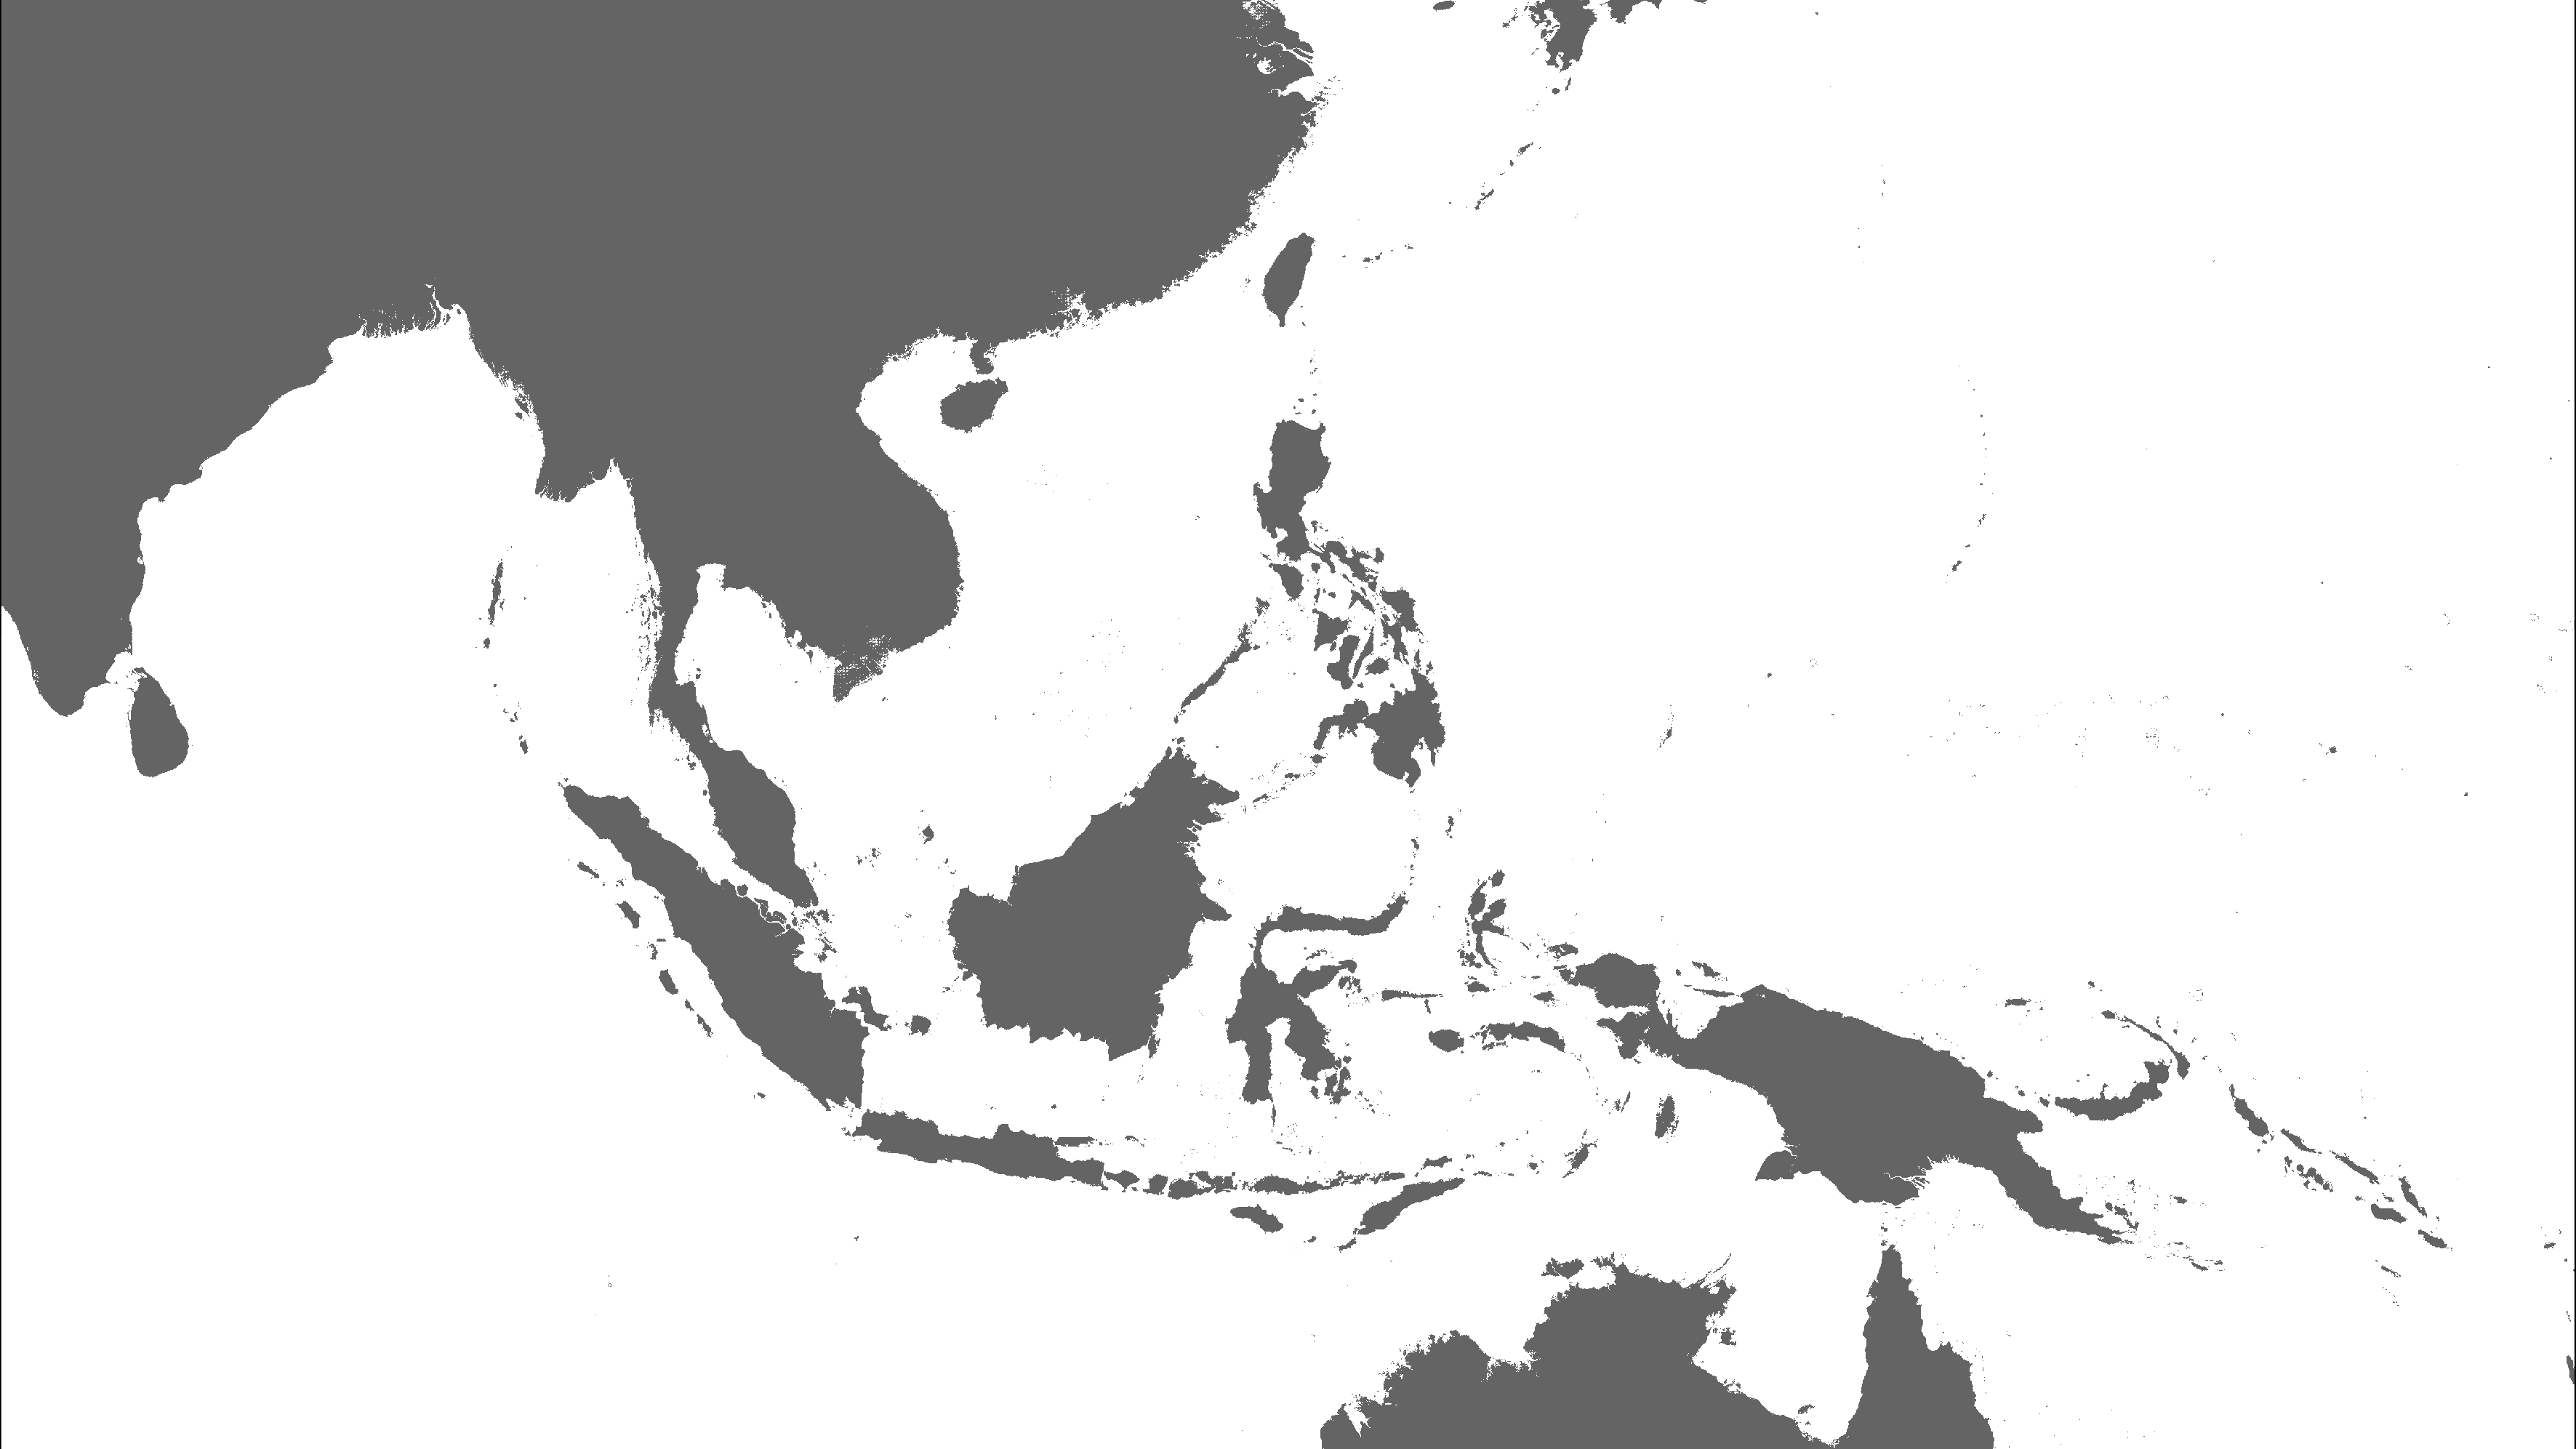
\includegraphics[width=\paperwidth]{../images/se-asia-present-widescreen.png}}
\usebackgroundtemplate{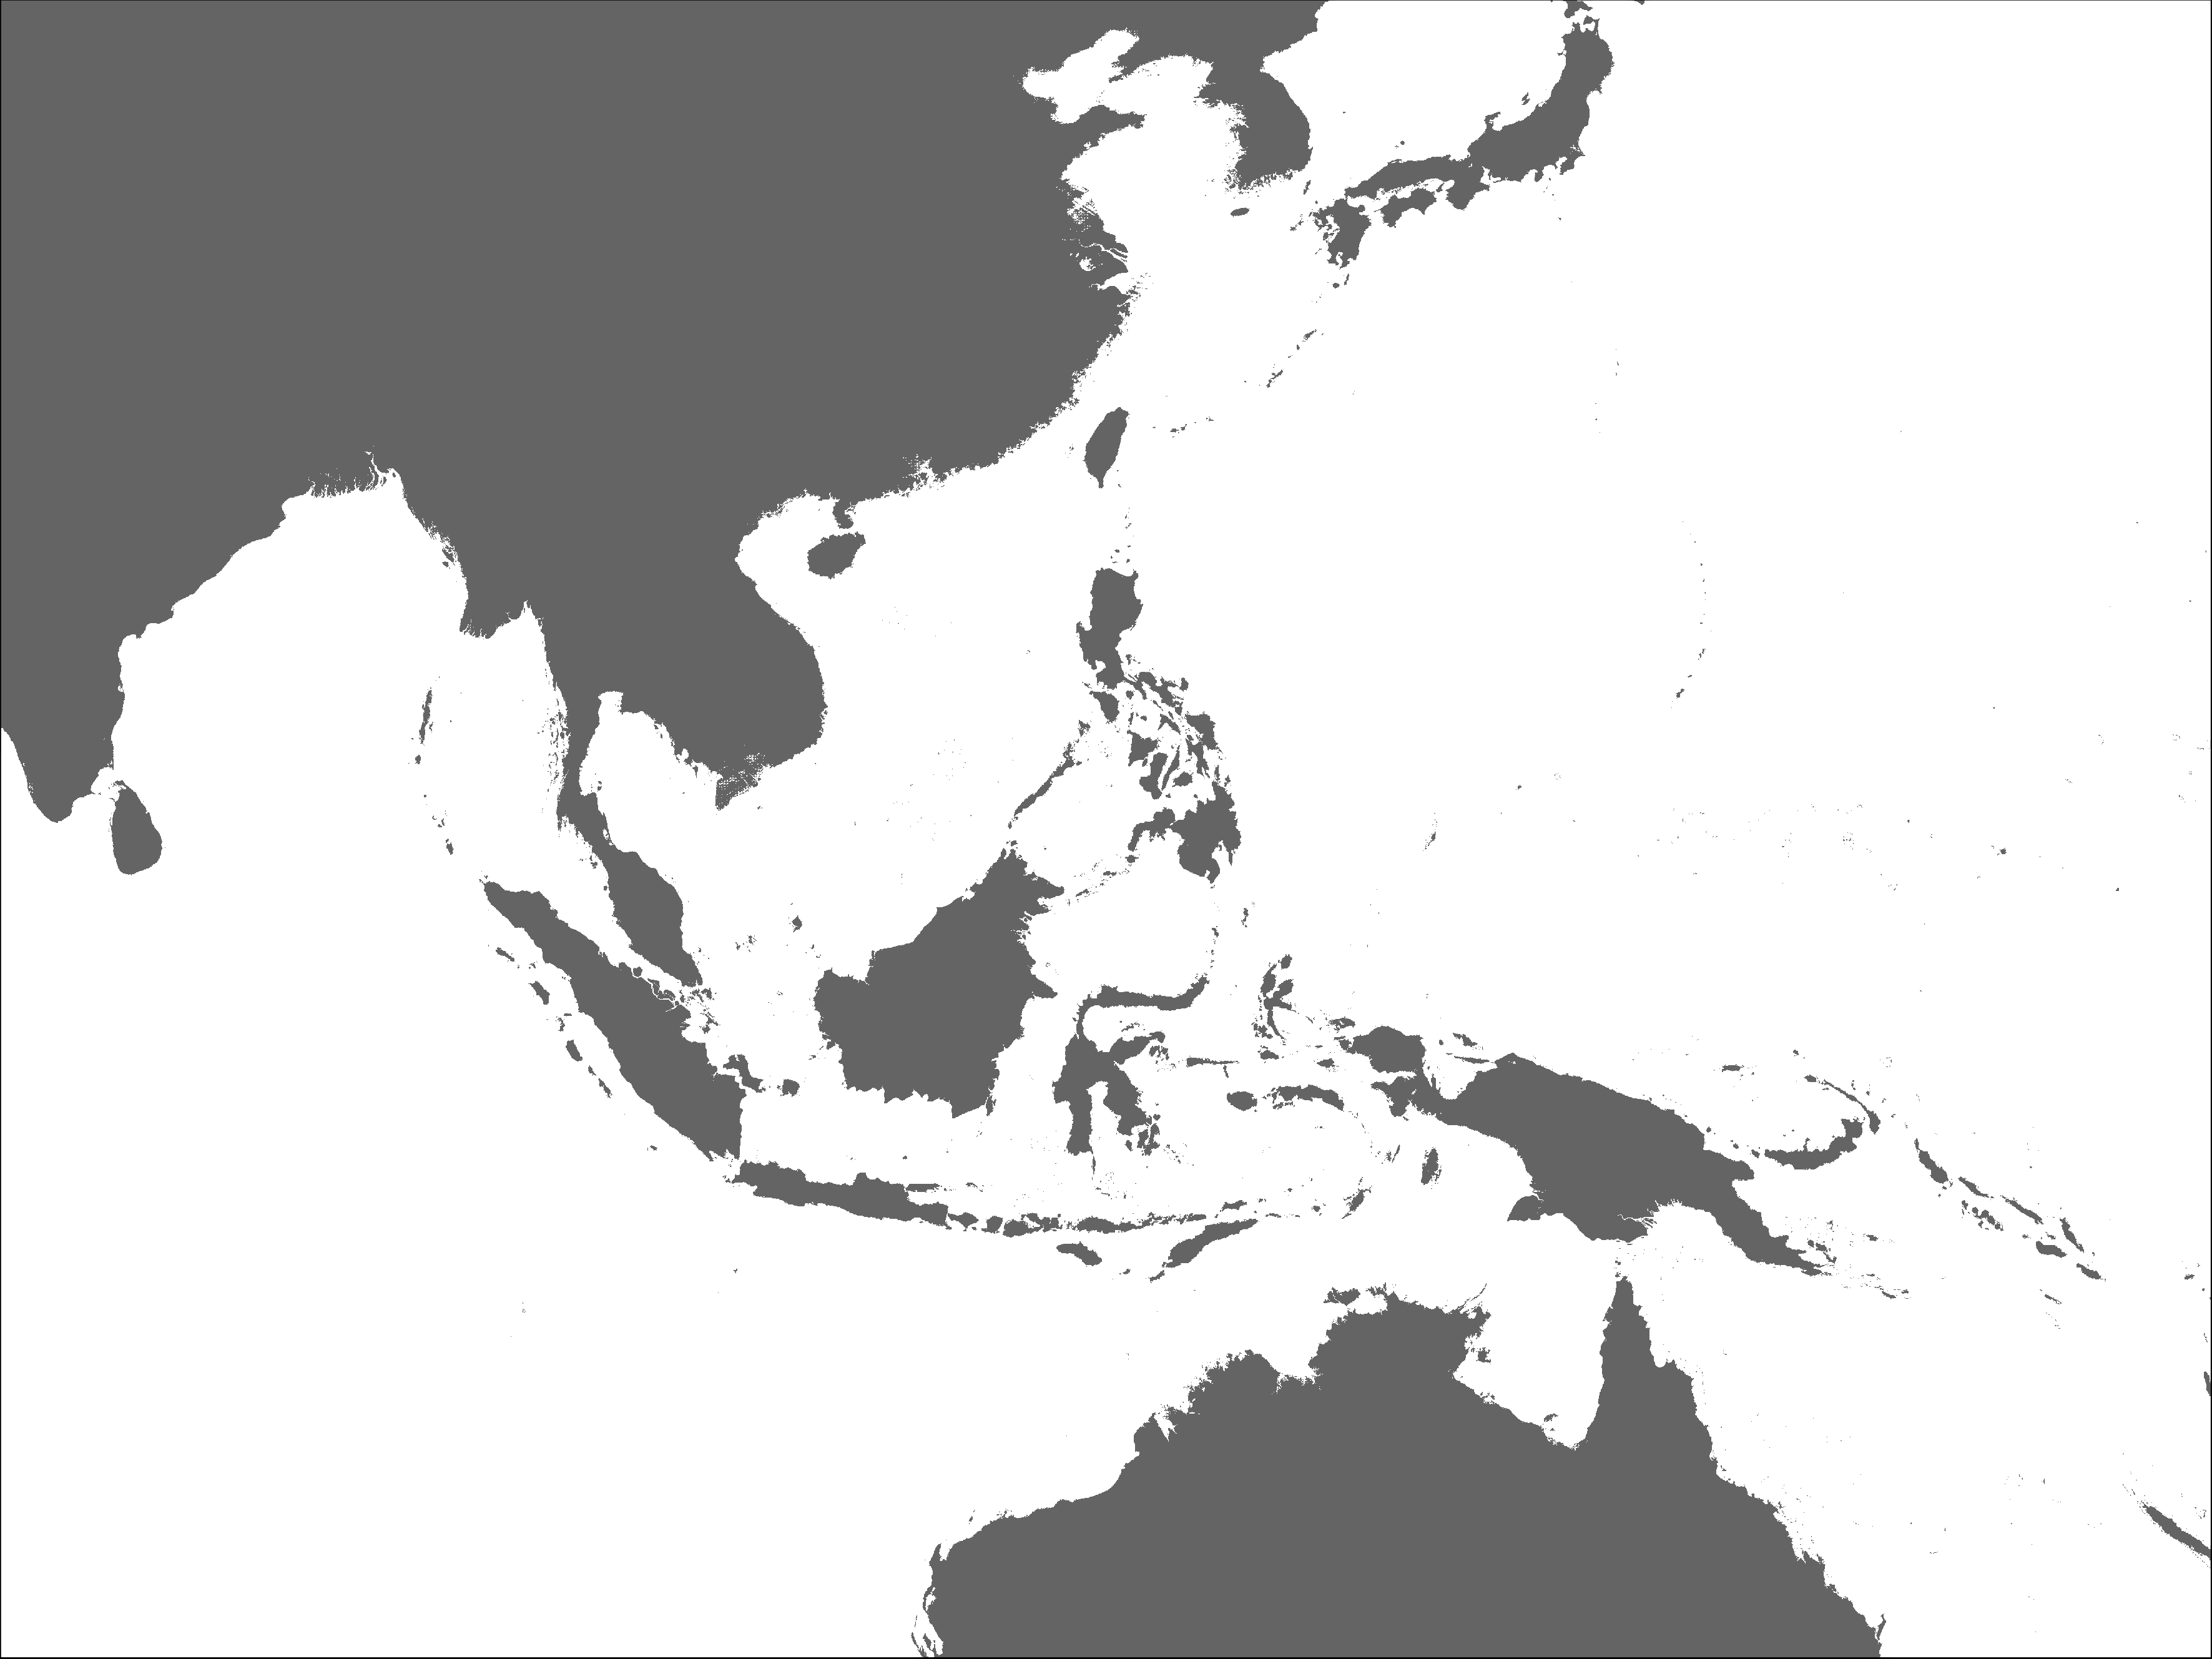
\includegraphics[width=\paperwidth]{../images/se-asia-present.png}}
\begin{frame}
    % \frametitle{Empirical applications}    
\end{frame}
}
{
% \usebackgroundtemplate{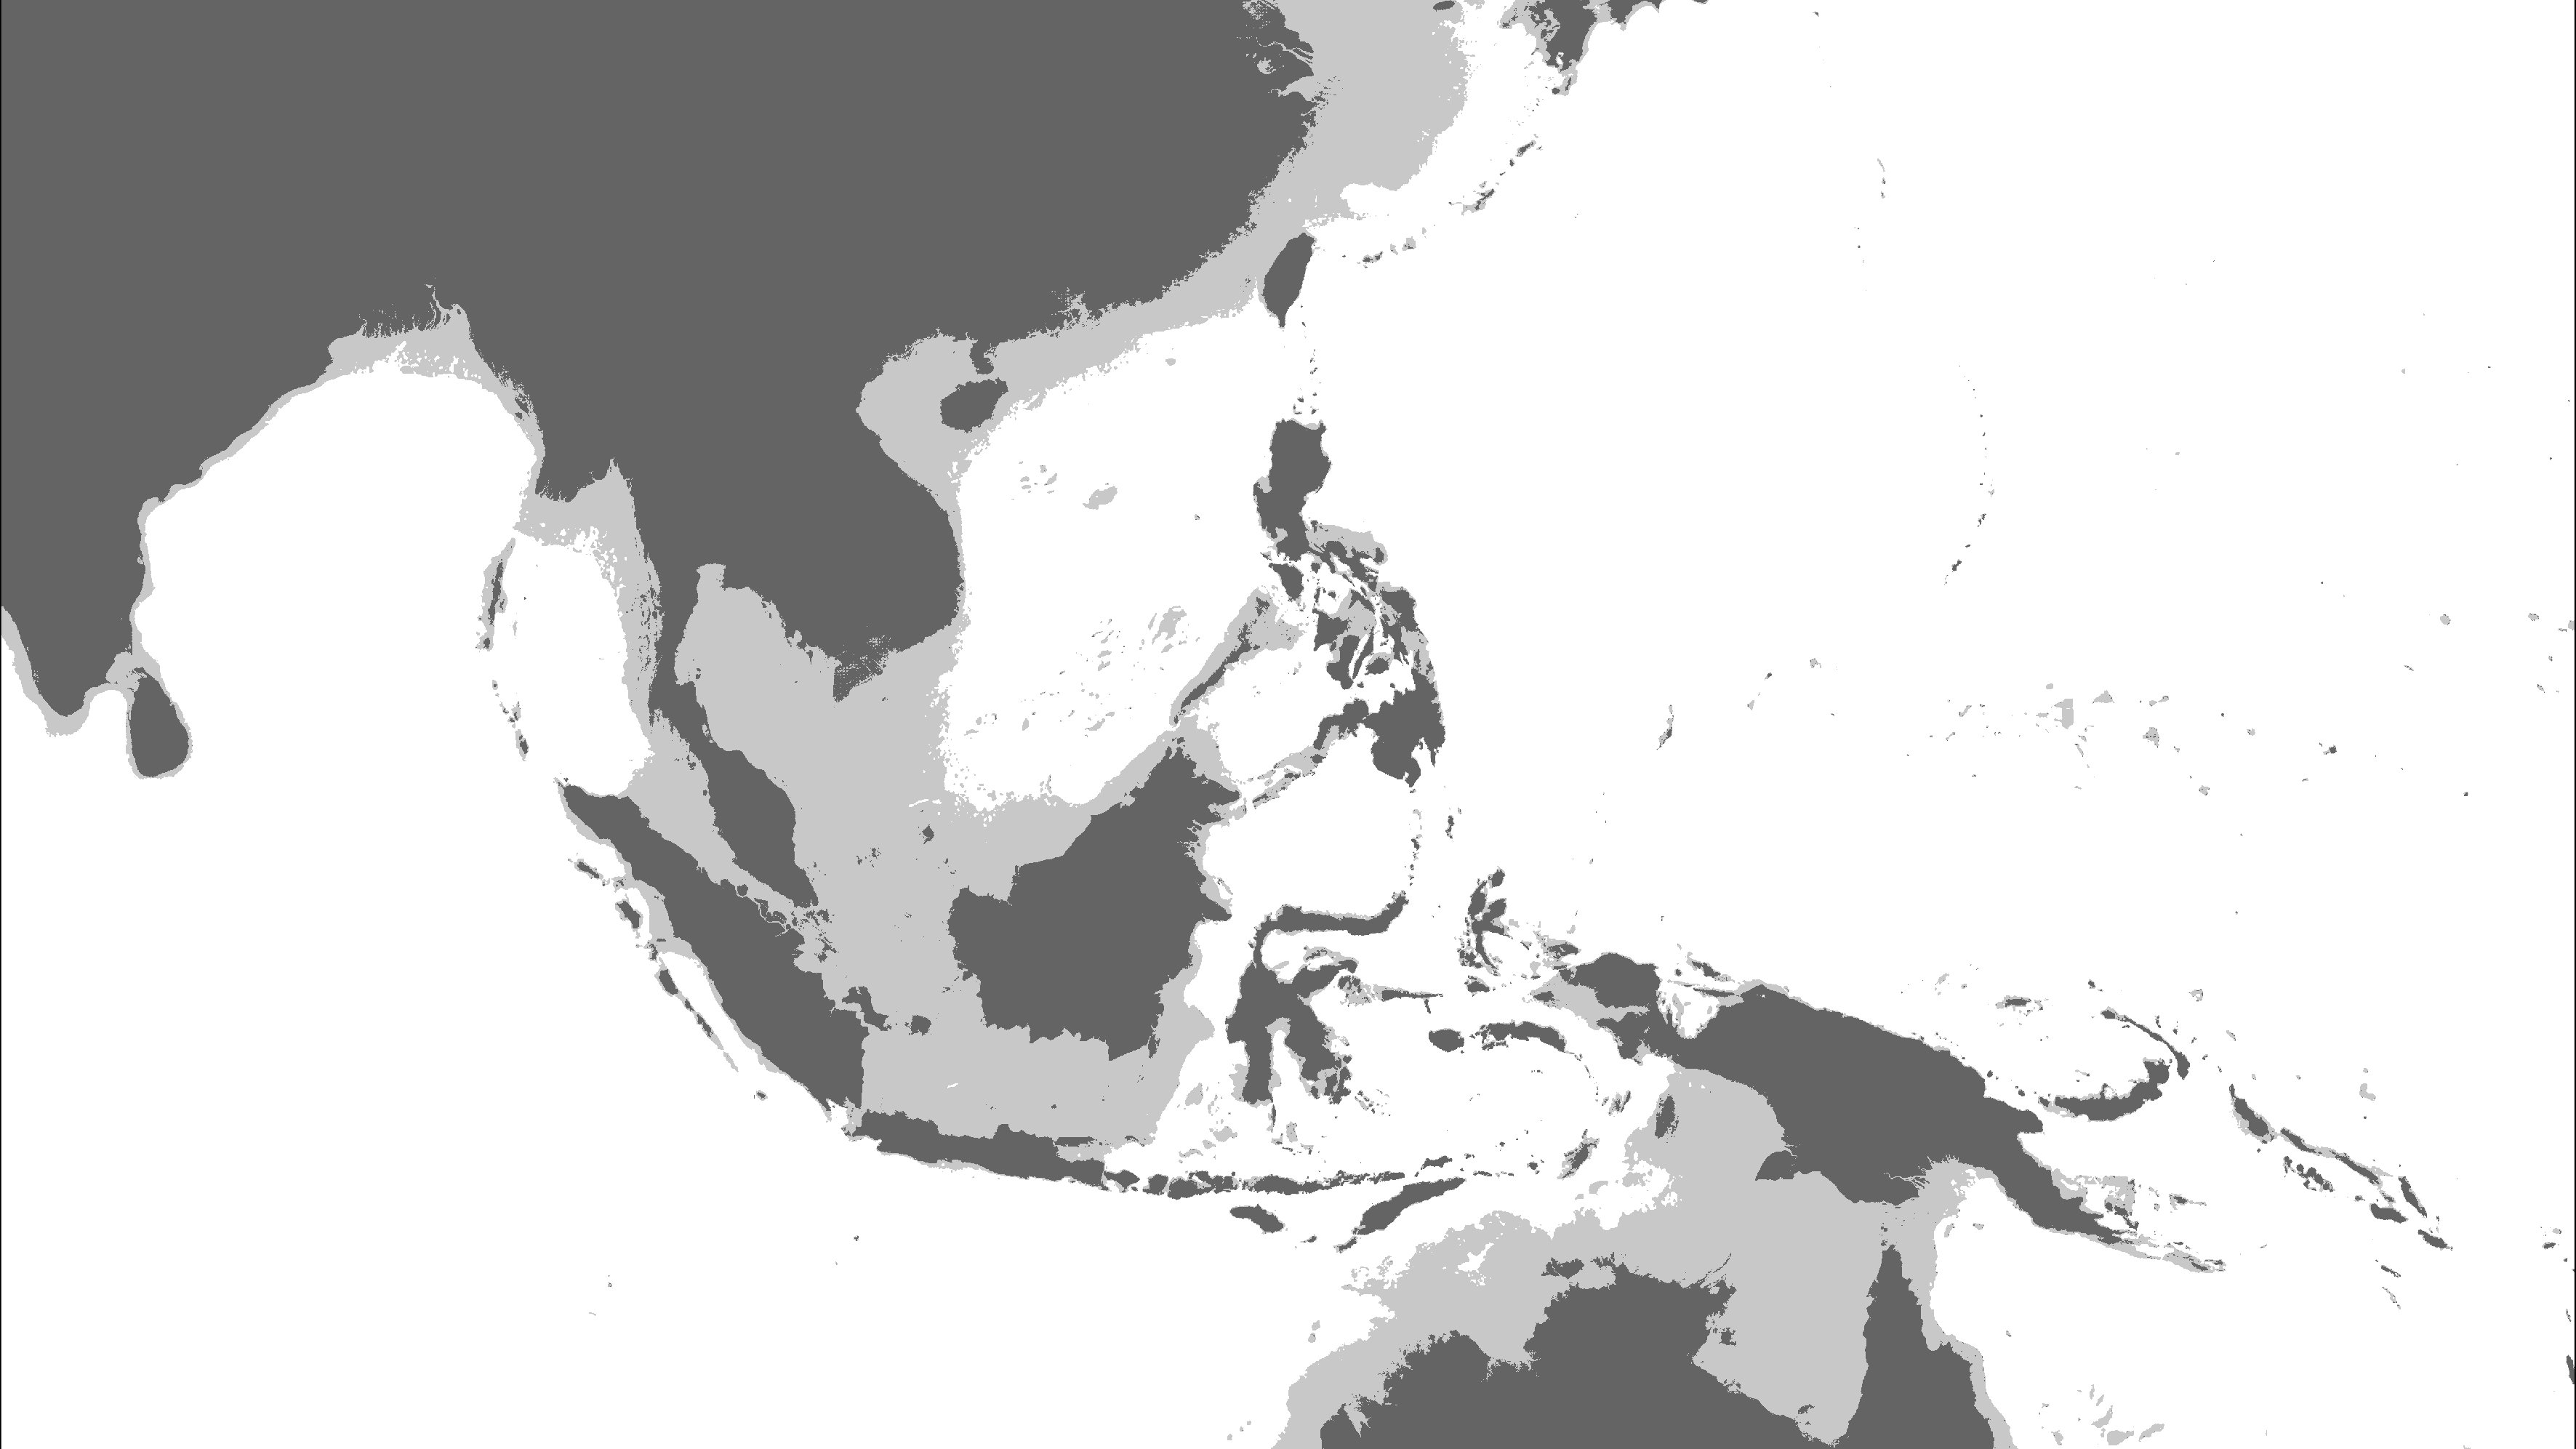
\includegraphics[width=\paperwidth]{../images/se-asia-120-widescreen.png}}
\usebackgroundtemplate{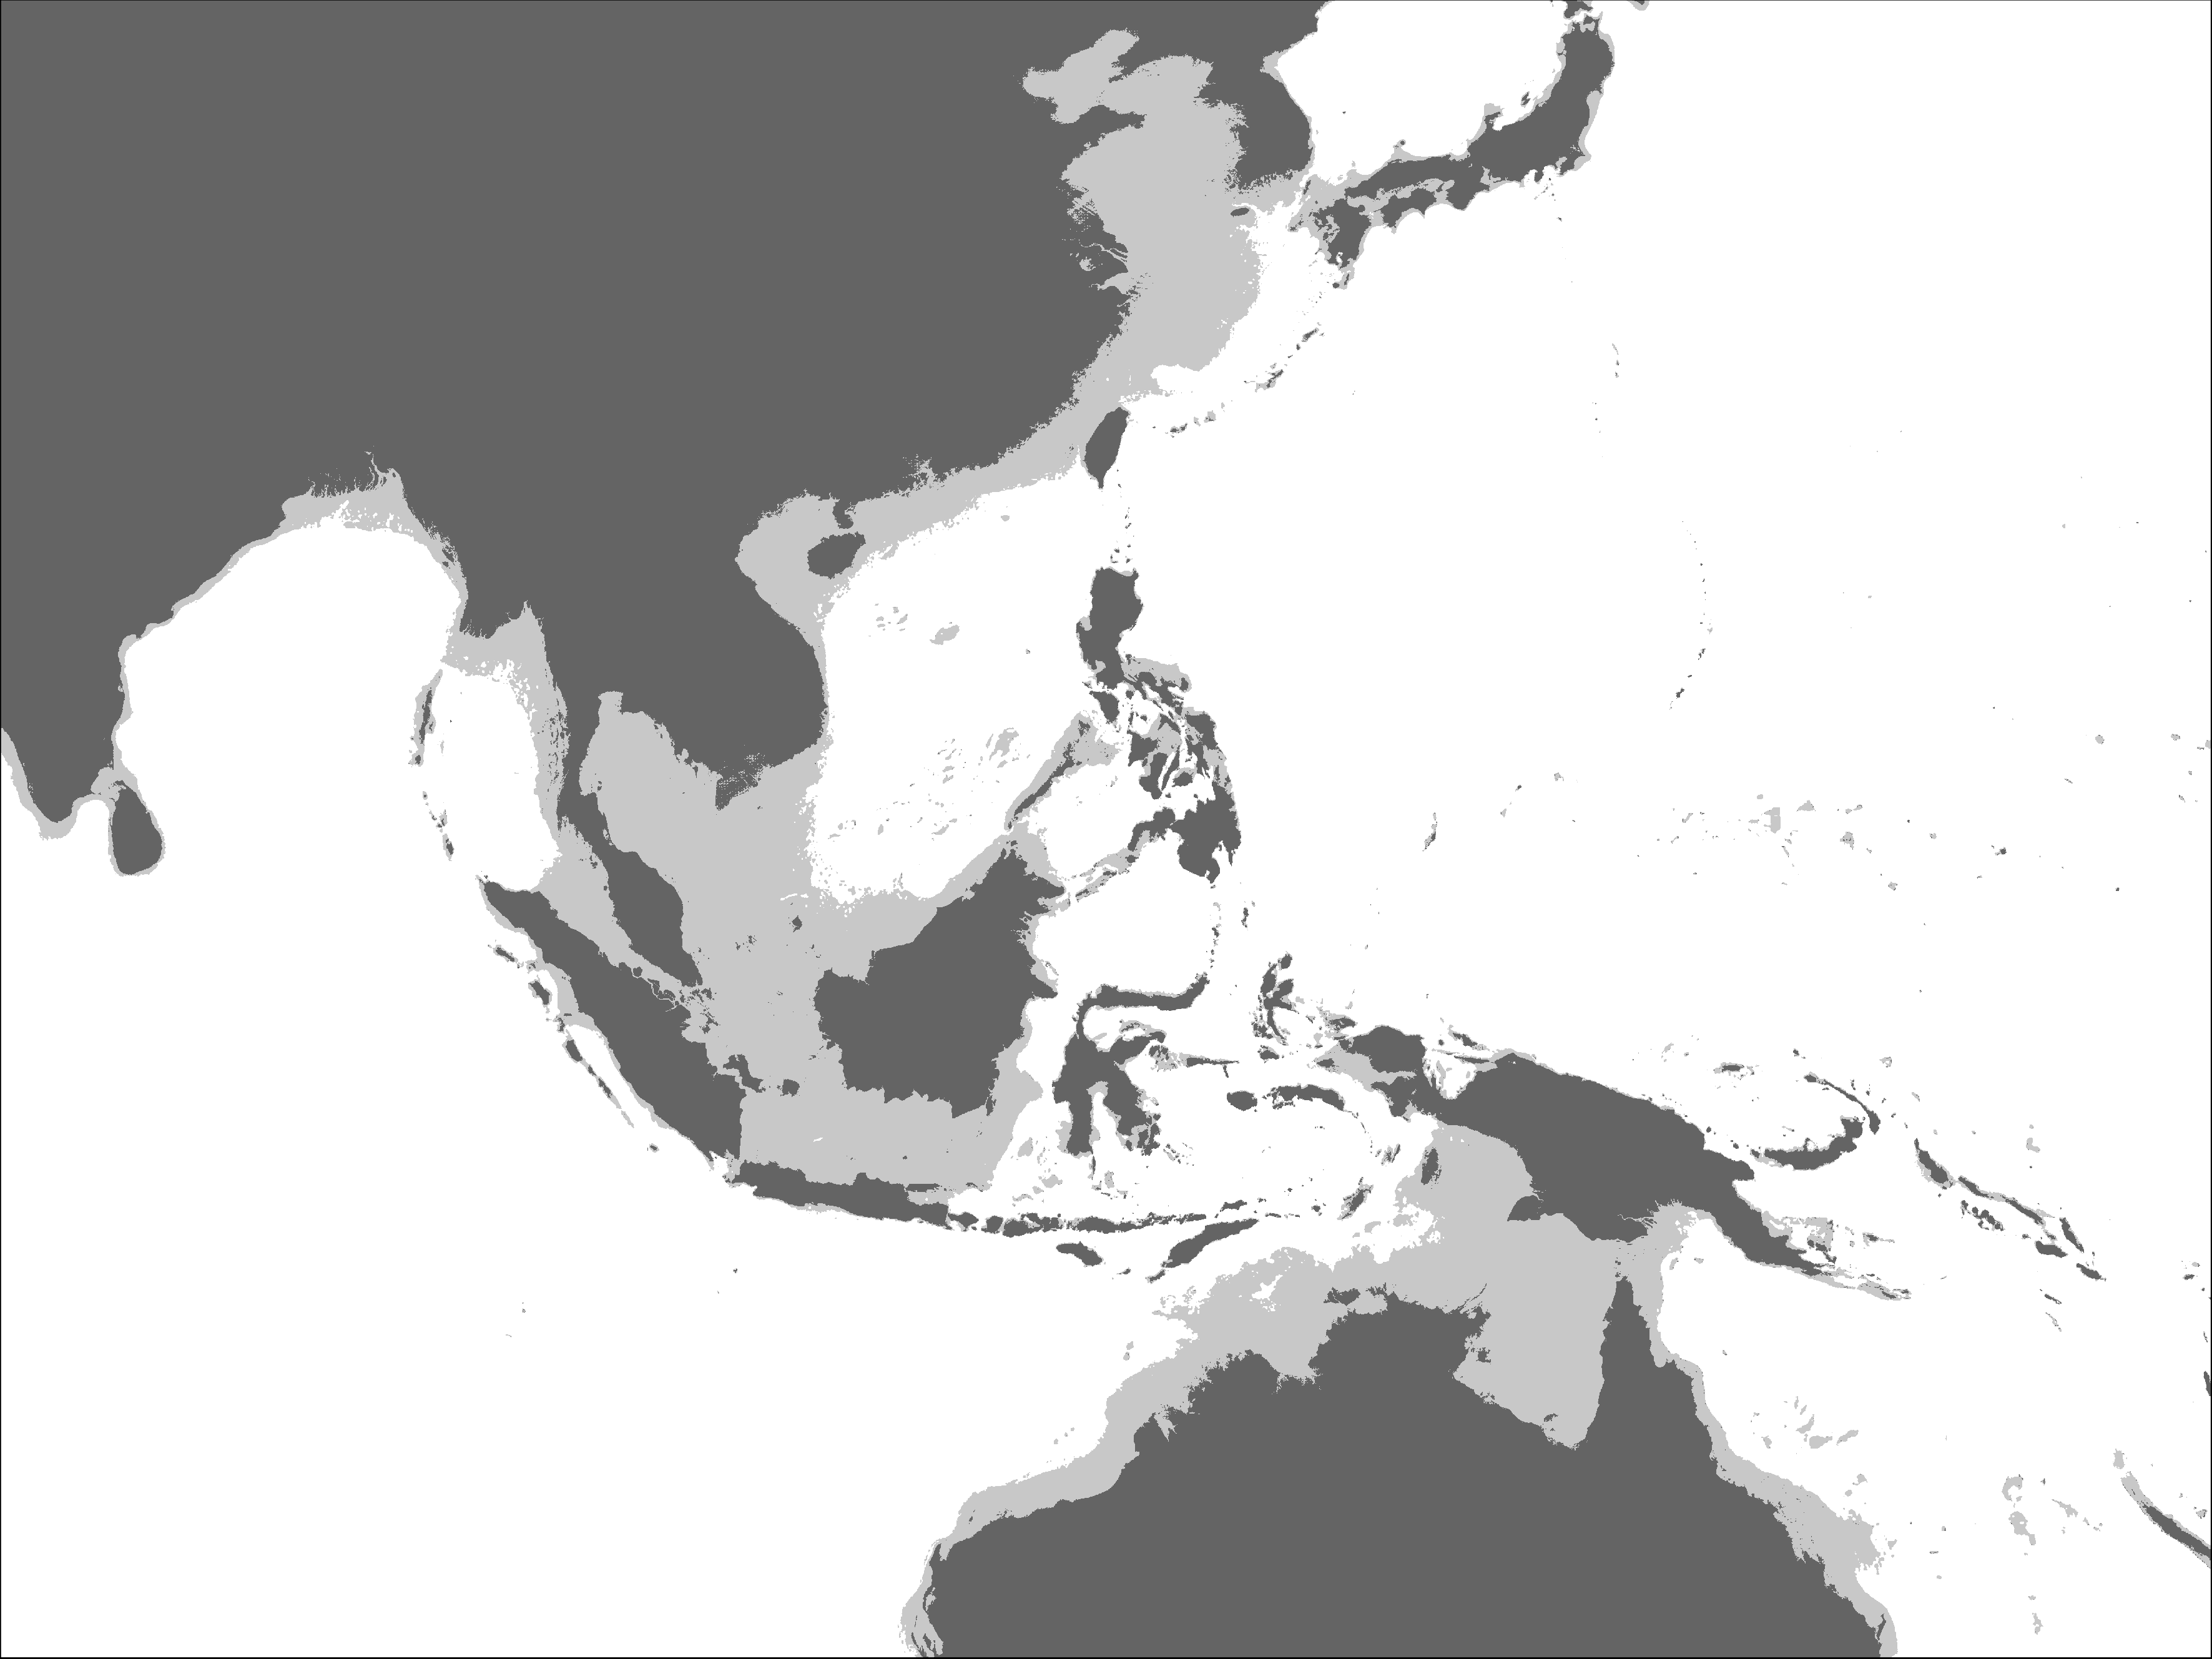
\includegraphics[width=\paperwidth]{../images/se-asia-120.png}}
\begin{frame}
    % \frametitle{Empirical applications}    
    \begin{columns}
        \column{0.56\textwidth}

        \vspace{6.5cm}

        \begin{uncoverenv}<3->
        \colorbox{white}{
            \begin{minipage}[t]{0.6\textwidth}
                \raggedright
                See a
                \href{https://youtu.be/mLNLRdbu5W8}{sea-level animation of SE Asia here}
            \end{minipage}
        }
        \end{uncoverenv}

        \ \\

        \column{0.4\textwidth}

        \vspace{-2cm}

        \begin{uncoverenv}<2->
        \colorbox{white}{
            \begin{minipage}[t]{1.0\textwidth}
                \raggedright
                \textbf{Did repeated fragmentation of islands during
                    inter-glacial rises in sea level promote diversification?}
            \end{minipage}
        }
        \end{uncoverenv}
    \end{columns}
\end{frame}
}

{
\usebackgroundtemplate{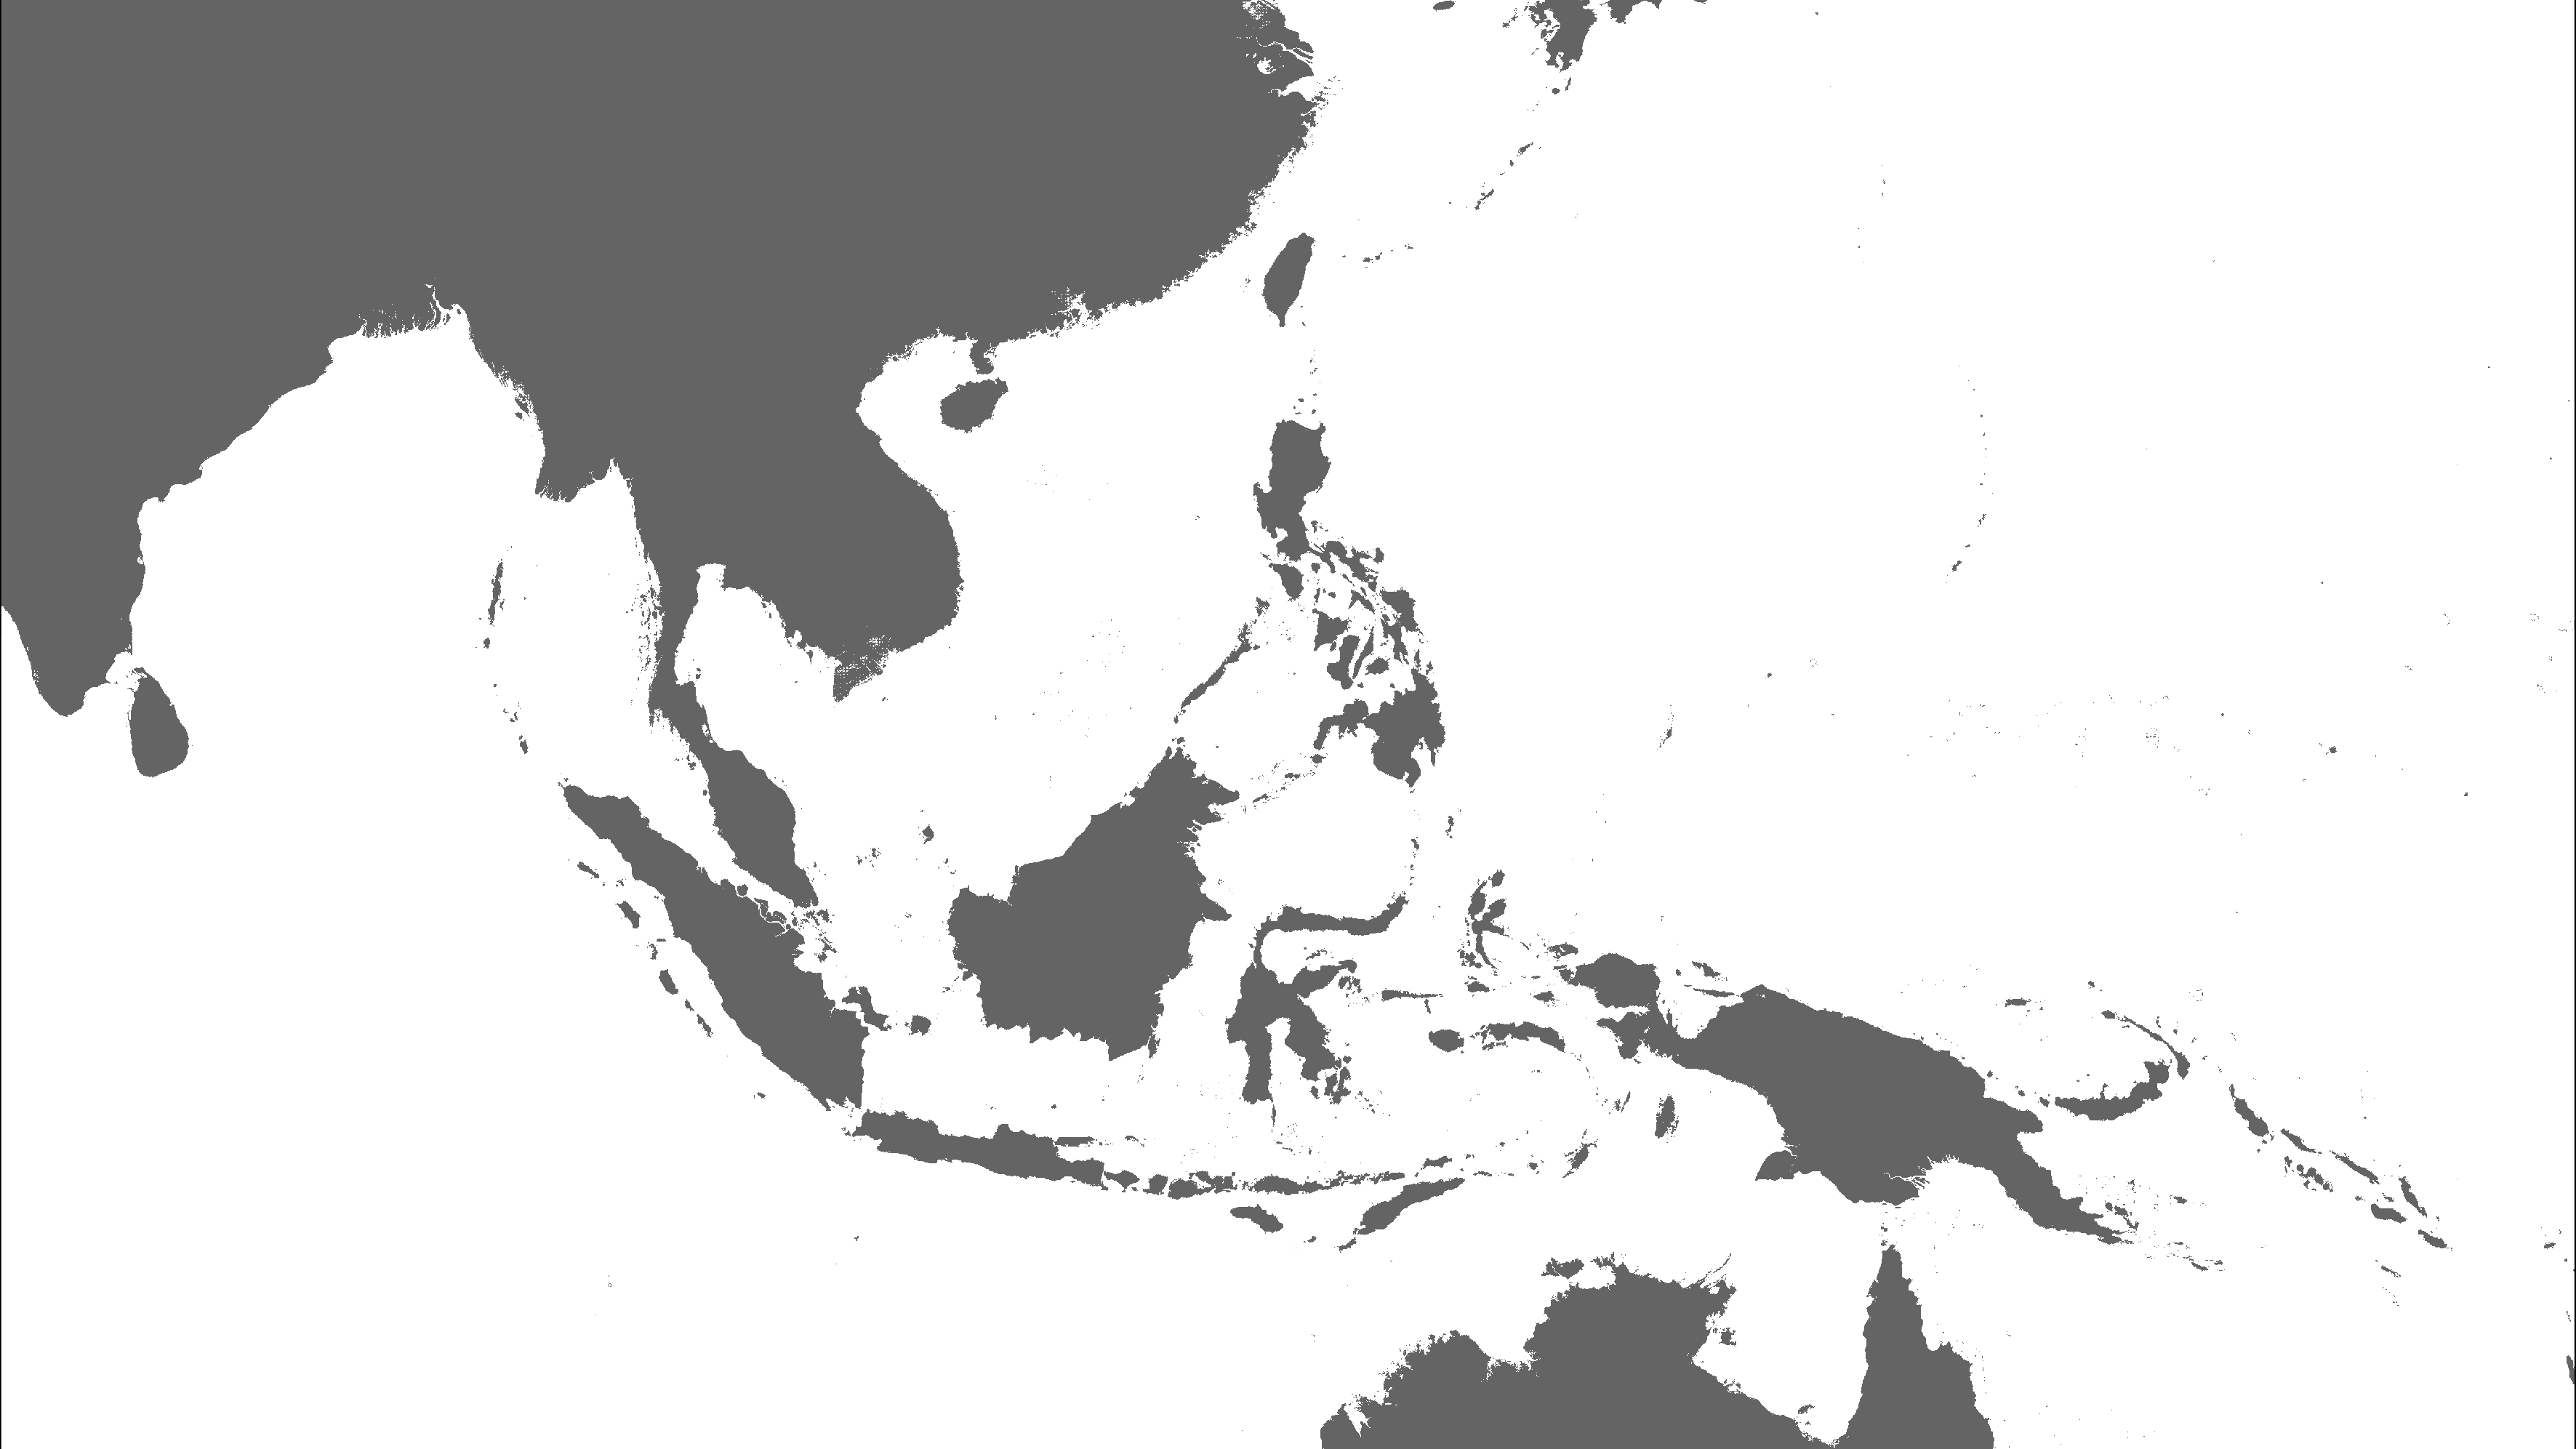
\includegraphics[width=\paperwidth]{../images/se-asia-present-widescreen.png}}
% \usebackgroundtemplate{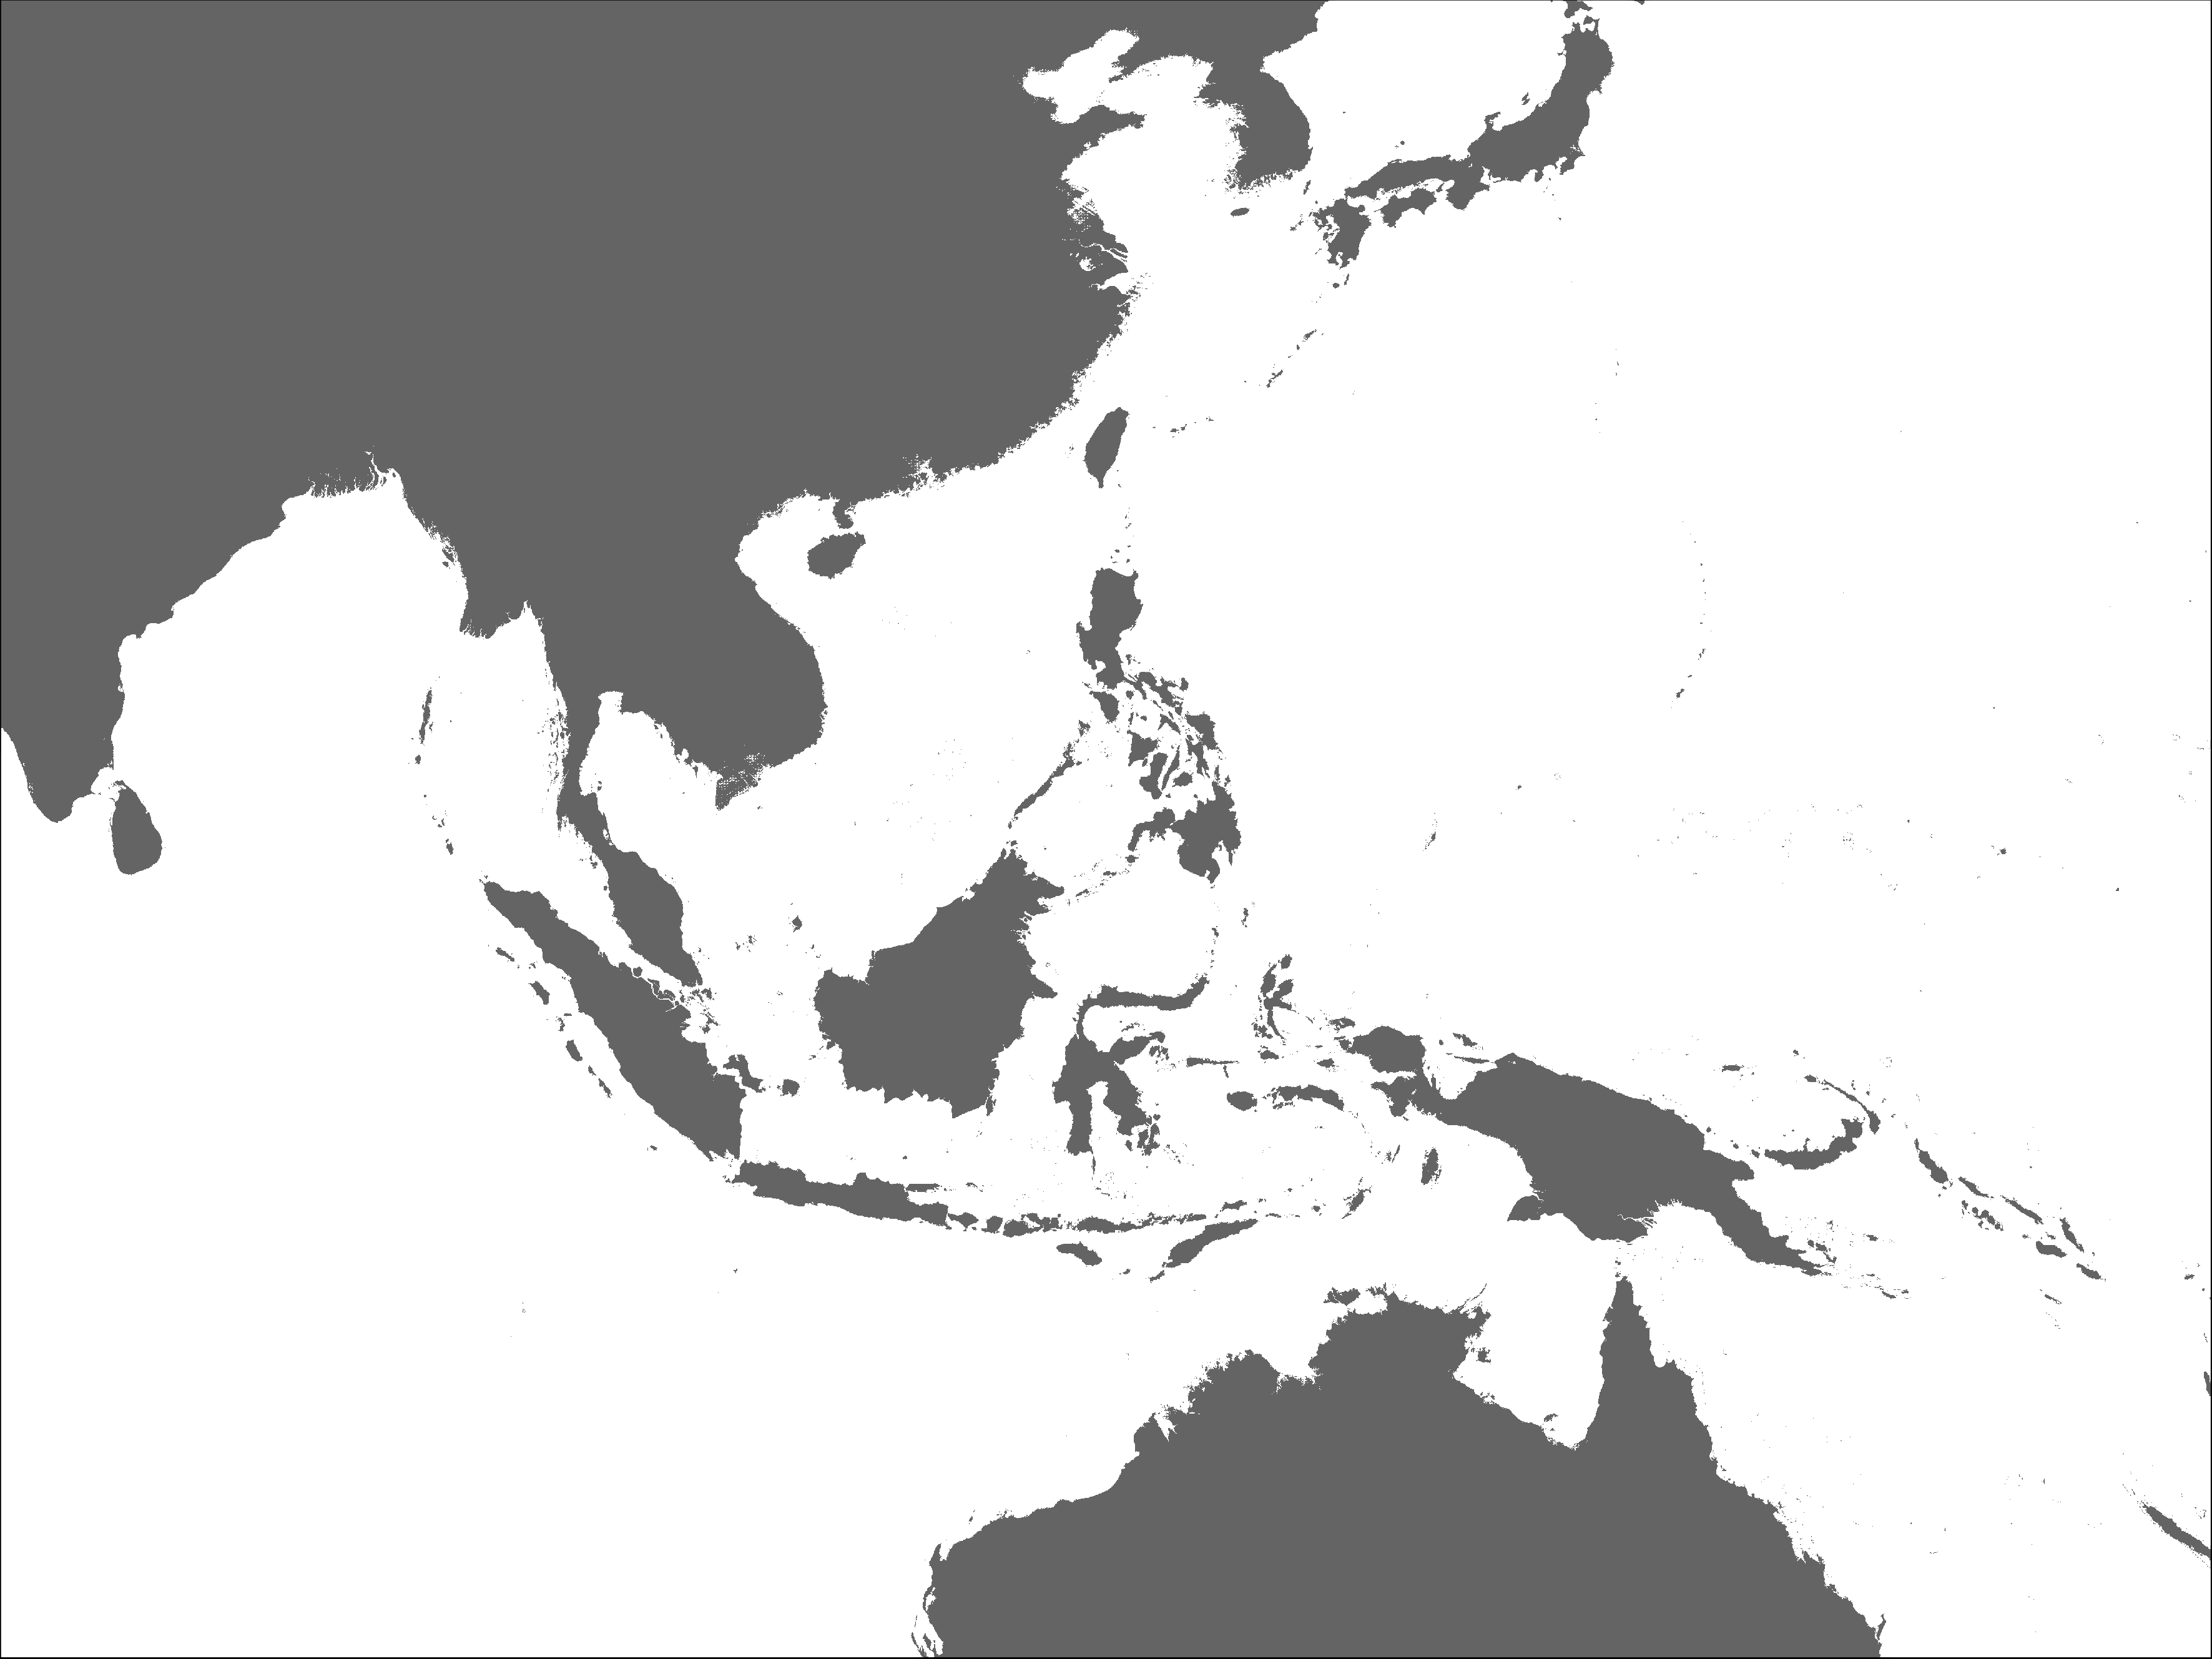
\includegraphics[width=\paperwidth]{../images/se-asia-present.png}}
\begin{frame}
    % \frametitle{Empirical applications}    
\end{frame}
}
{
\usebackgroundtemplate{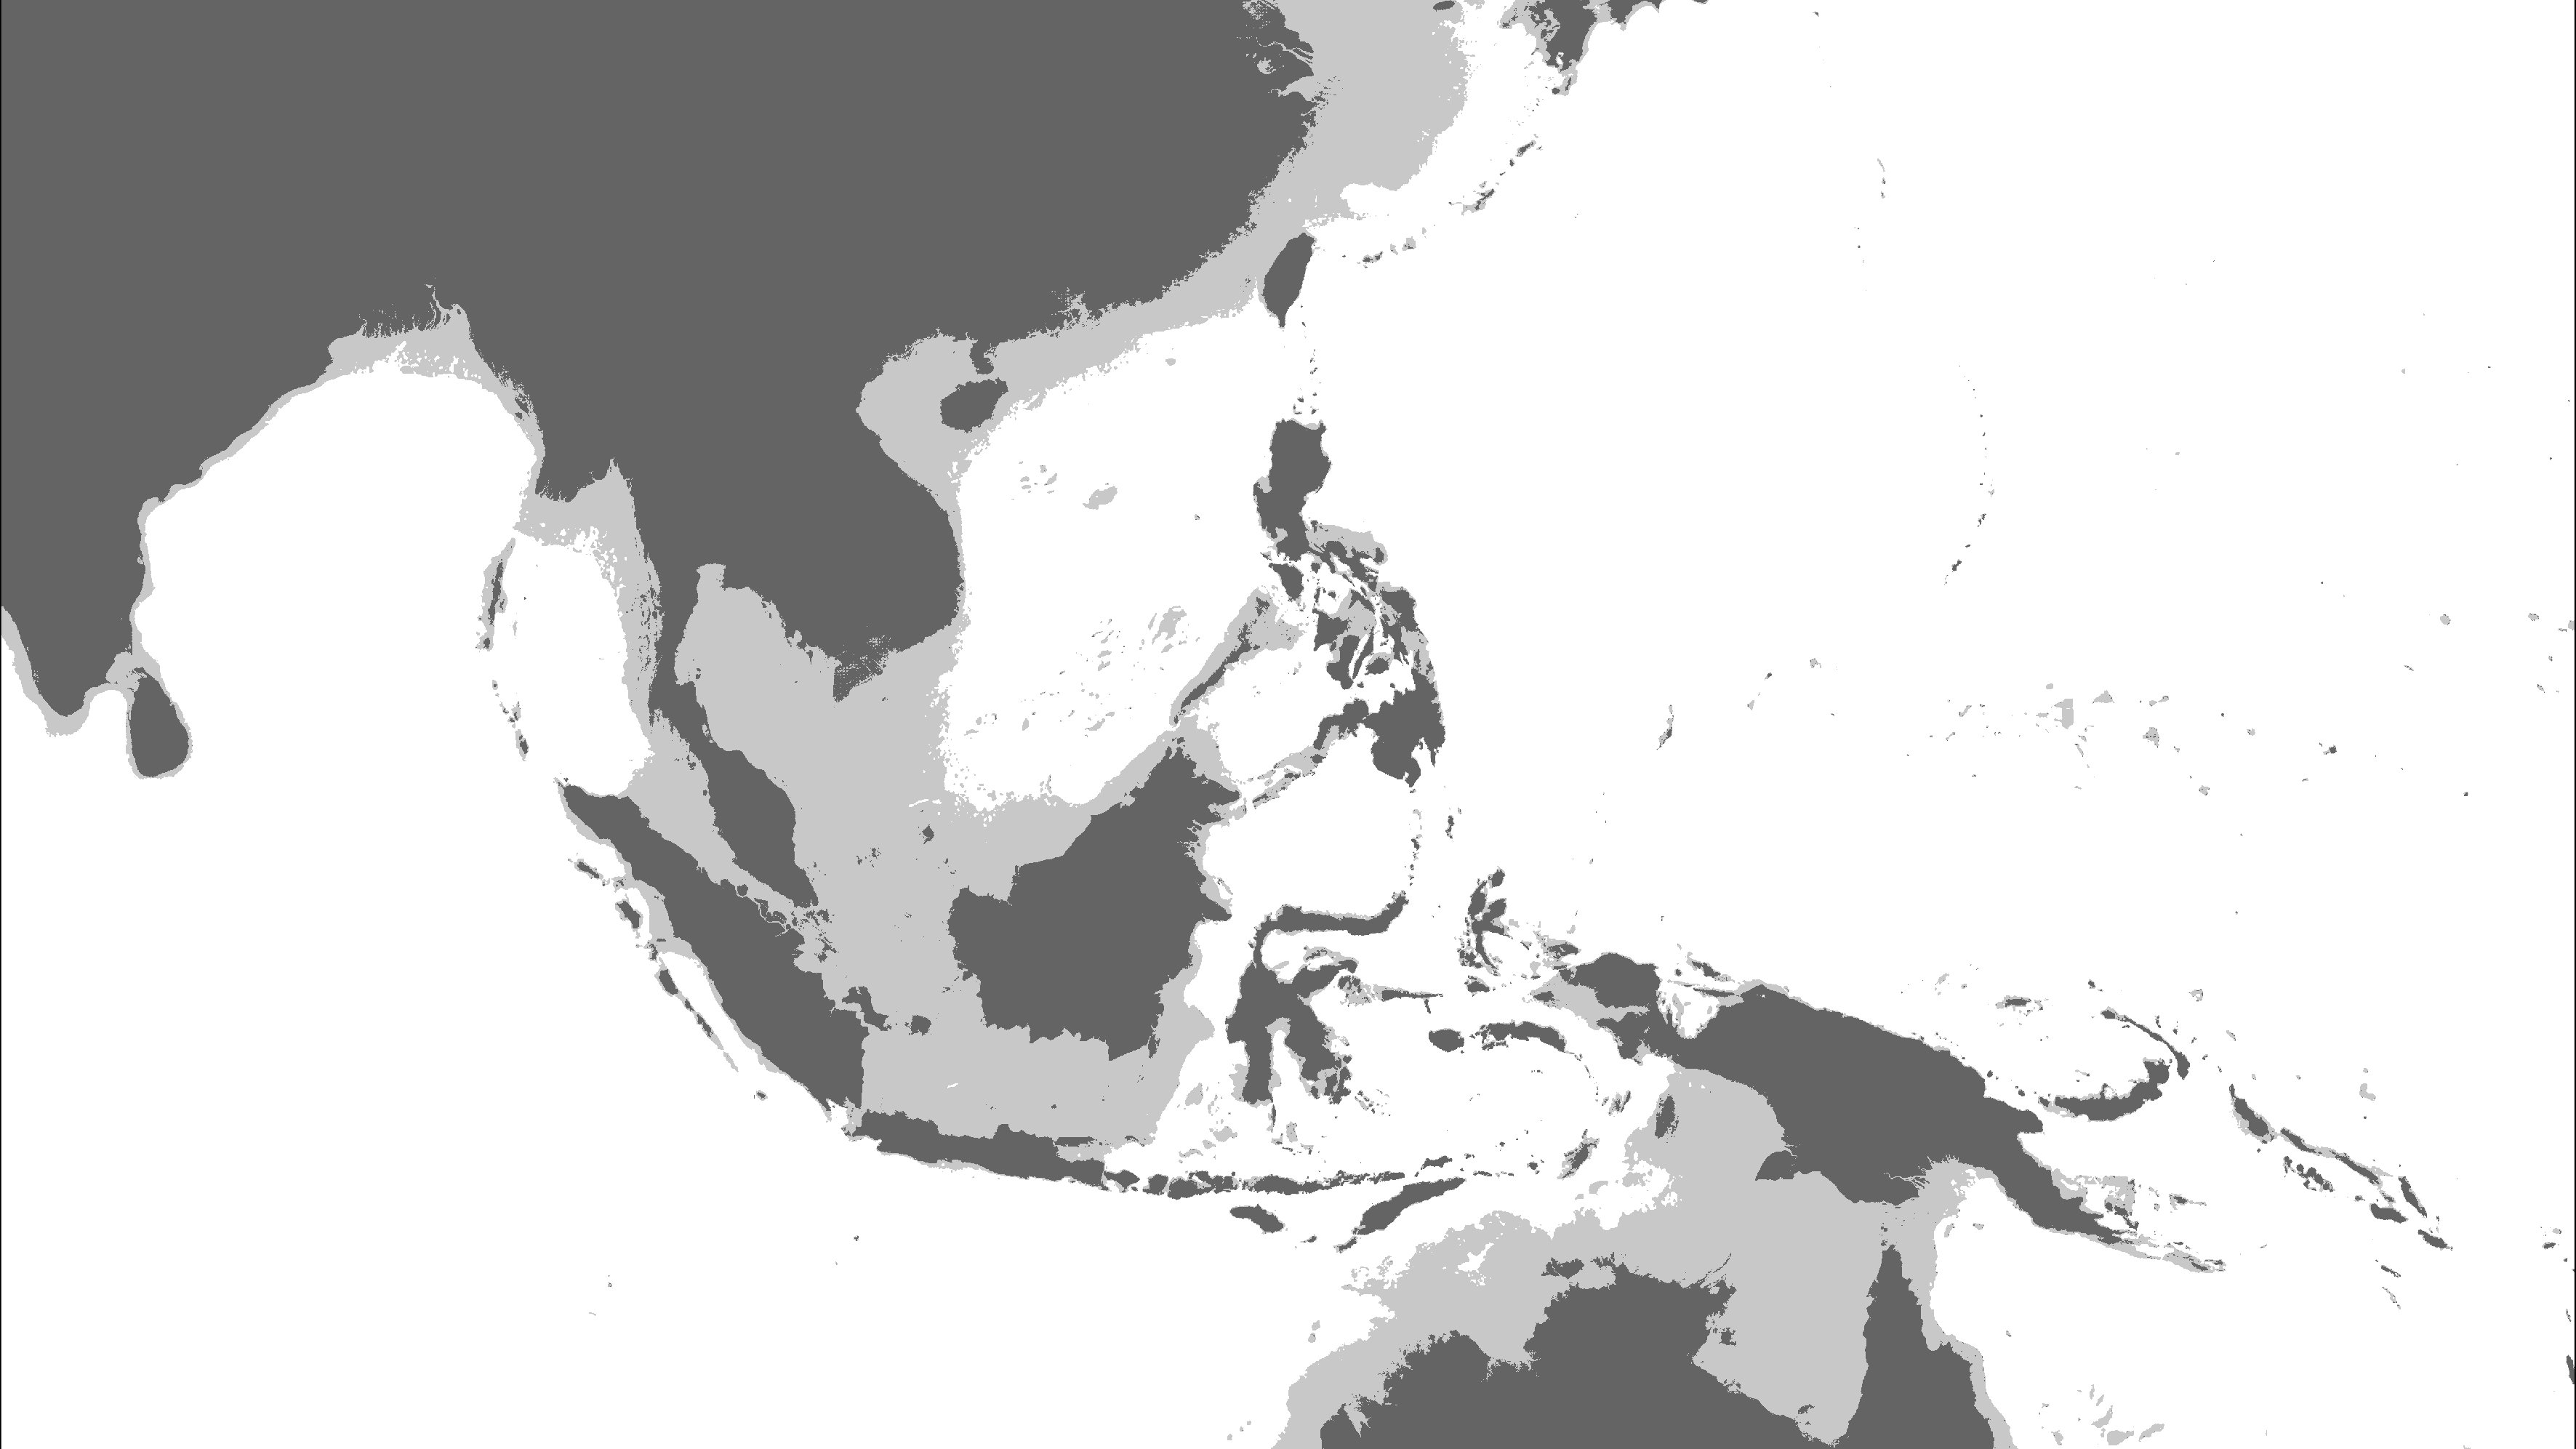
\includegraphics[width=\paperwidth]{../images/se-asia-120-widescreen.png}}
% \usebackgroundtemplate{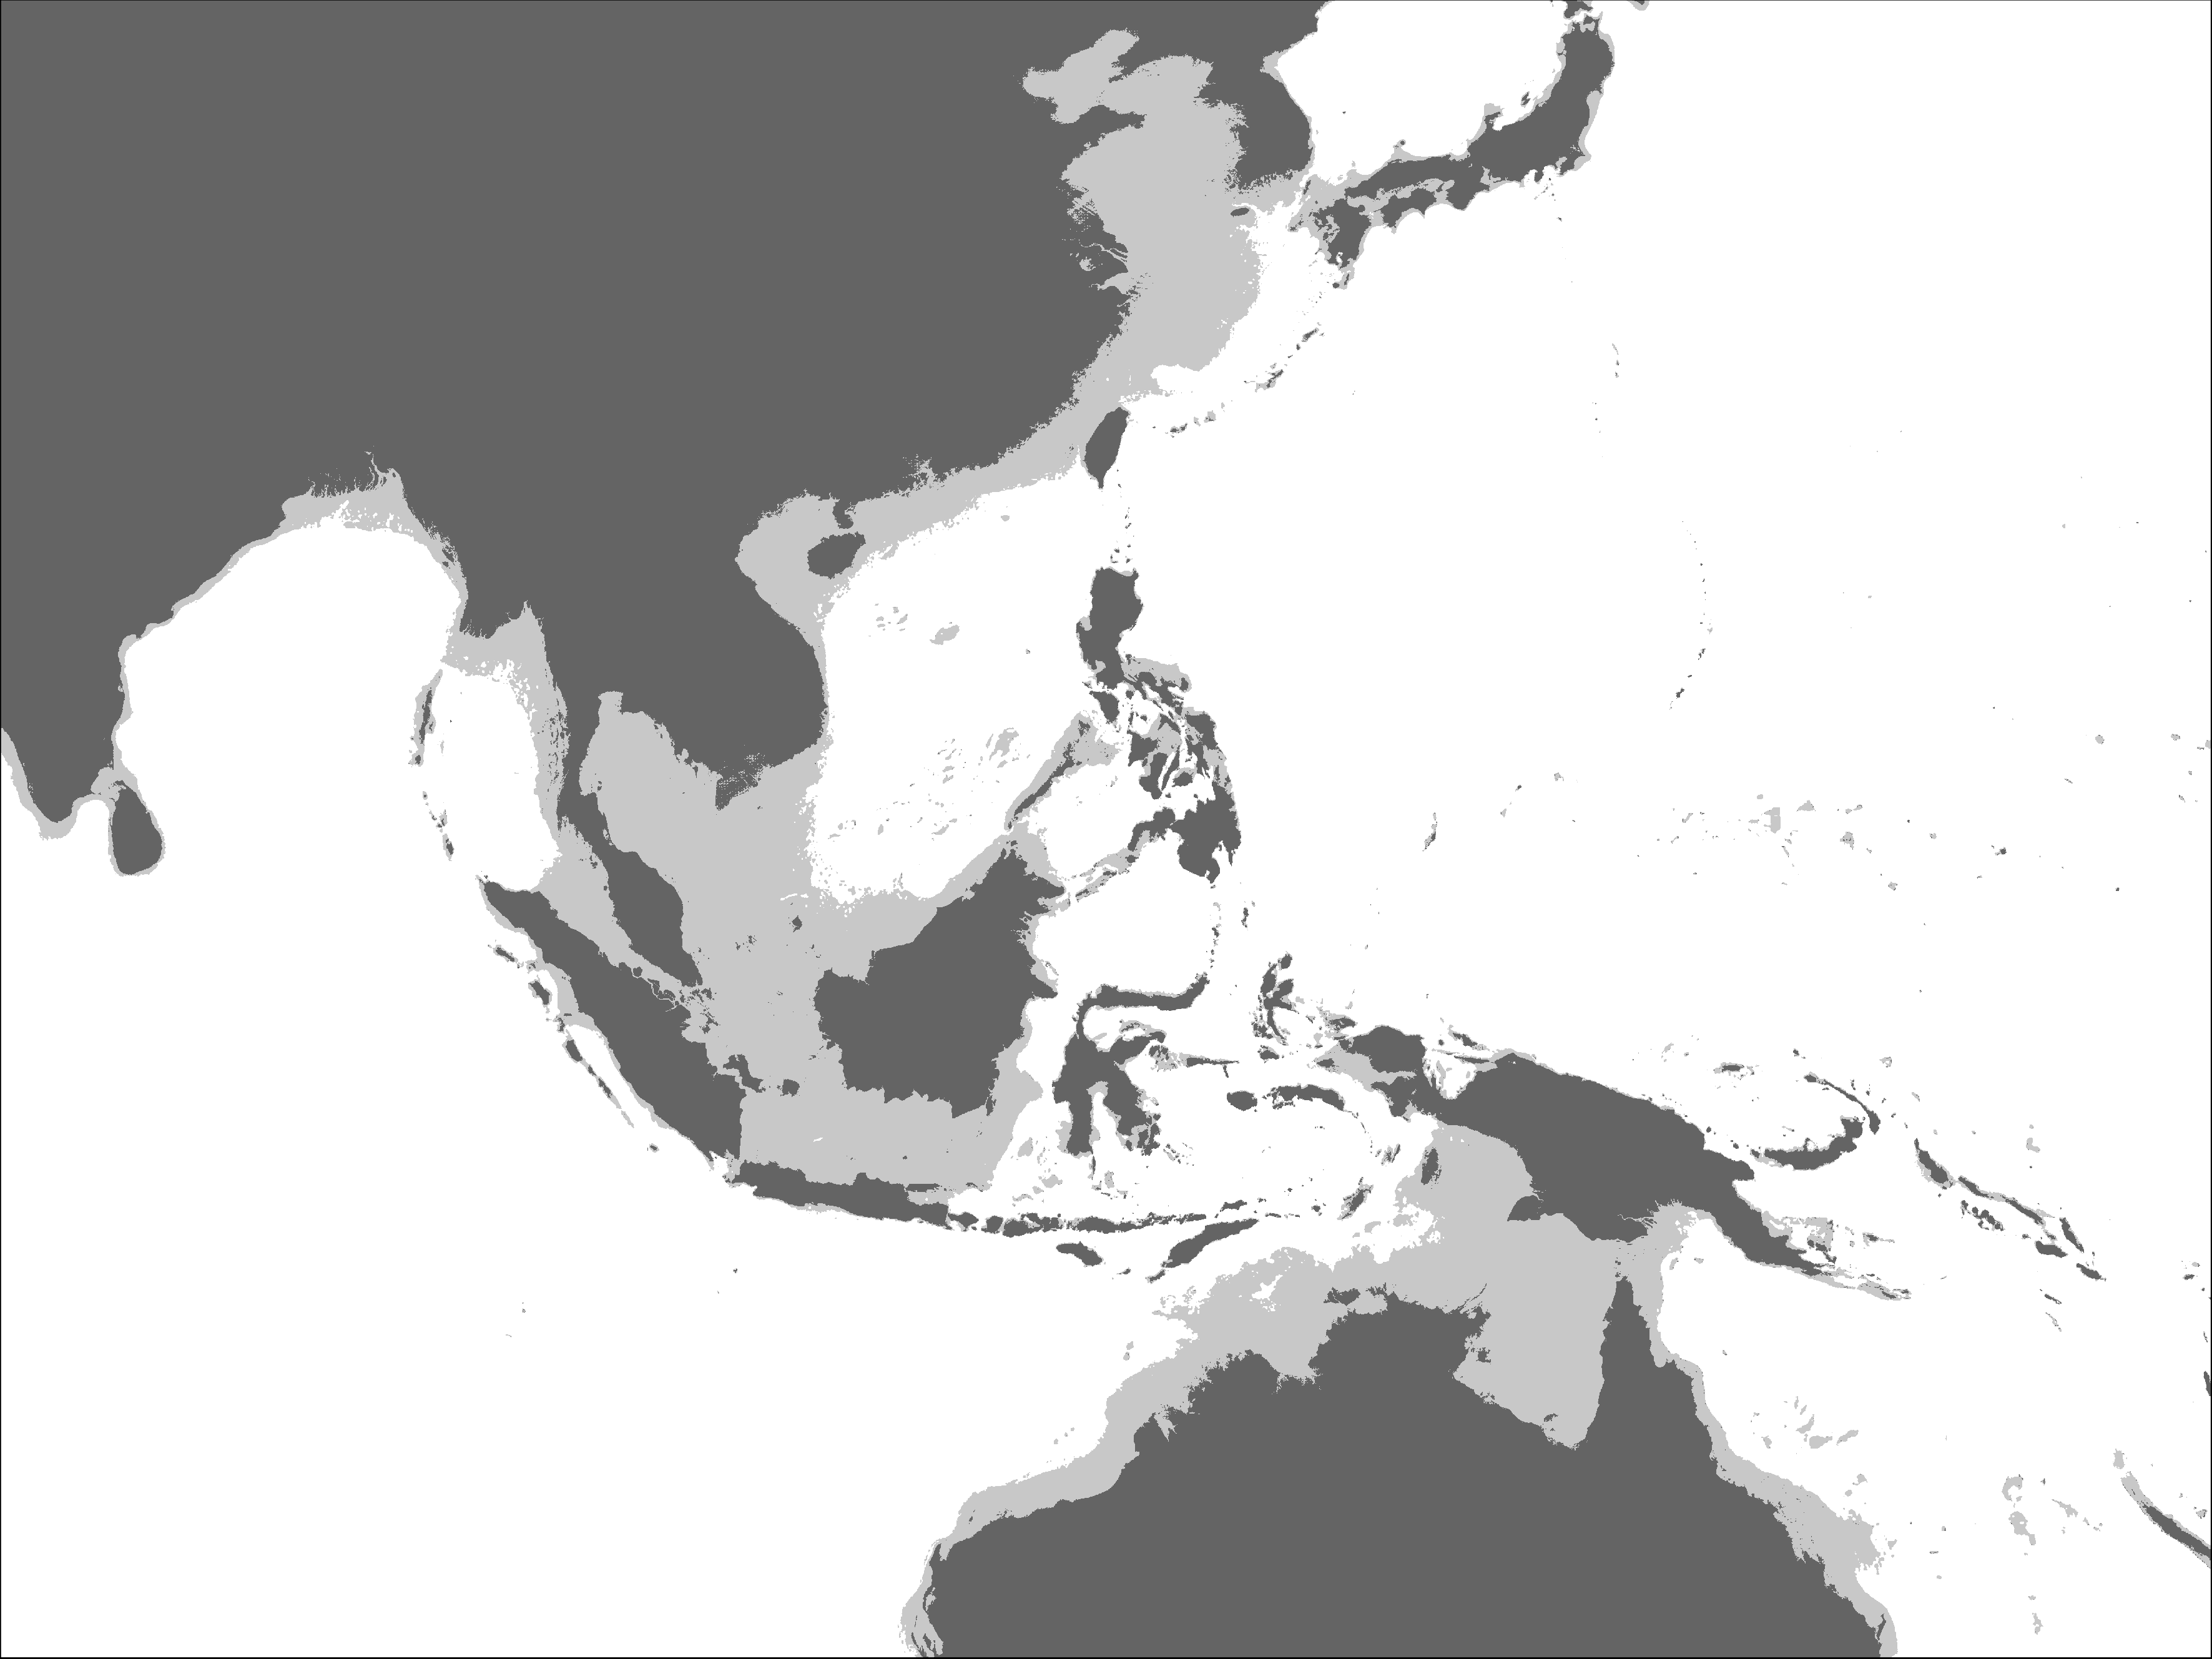
\includegraphics[width=\paperwidth]{../images/se-asia-120.png}}
\begin{frame}
    % \frametitle{Empirical applications}    
    \begin{columns}
        \column{0.56\textwidth}

        \vspace{6.7cm}

        \begin{uncoverenv}<3->
        \colorbox{white}{
            \begin{minipage}[t]{0.45\textwidth}
                \raggedright
                \href{https://youtu.be/mLNLRdbu5W8}{Click here for a sea-level animation of SE Asia youtu.be/mLNLRdbu5W8}
            \end{minipage}
        }
        \end{uncoverenv}

        \ \\

        \column{0.4\textwidth}

        \vspace{-2cm}

        \begin{uncoverenv}<2->
        \colorbox{white}{
            \begin{minipage}[t]{1.0\textwidth}
                \raggedright
                \textbf{Did fragmentation of islands promote diversification?}
            \end{minipage}
        }
        \end{uncoverenv}
    \end{columns}
\end{frame}
}

% \begin{frame}
    \begin{description}
        \item<1->[``Species-pump'' Hypothesis] 
            Repeated climate-driven fragmentation of the Philippine Islands was
            a primary mechanism of speciation for terrestrial fauna
        \item<2->[Prediction]
            Taxa co-distributed across islands within the same Pleistocene
            aggregate island complex (PAIC) will have divergence times that
            tend to be clustered around times when sea levels fragmented the
            islands
    \end{description}
\end{frame}


\begin{frame}[c]
    % \frametitle{Violating independent divergences}

%% This is a tikz file
\tikzset{node lower left/.style={font=\small,anchor=north east,text height=0.240cm,text depth=0.068cm,inner sep=0.03cm},
leaf/.style={font=\small,anchor=west,text height=0.240cm,text depth=0.068cm},
node upper left/.style={font=\small,anchor=south east,text height=0.240cm,text depth=0.068cm,inner sep=0.03cm},
bracket label/.style={font=\small,anchor=west,text height=0.240cm,text depth=0.068cm,inner sep=0.1cm},
node upper right/.style={font=\small,anchor=south west,text height=0.240cm,text depth=0.068cm,inner sep=0.03cm},
node right/.style={font=\small,anchor=west,text height=0.240cm,text depth=0.068cm,inner sep=0.03cm},
branch/.style={font=\tiny,text height=0.144cm,text depth=0.041cm,inner sep=0.025cm},
root/.style={font=\small,anchor=east,text height=0.240cm,text depth=0.068cm},
node lower right/.style={font=\small,anchor=north west,text height=0.240cm,text depth=0.068cm,inner sep=0.03cm}}

\centering{
\resizebox{!}{\frametextheight}{%
\begin{tikzpicture}[ultra thick,inner sep=0.1cm]
%  4:\hspace{20mm}\includegraphics[width=15mm]{../images/phylopics/gekko-vittatus-4-yellow-shadow.png}
%  3
% +2:\hspace{20mm}\includegraphics[width=15mm]{../images/phylopics/gekko-vittatus-5-teal-shadow.png}
% ||
% |6:\hspace{20mm}\includegraphics[width=15mm]{../images/phylopics/gekko-vittatus-6-auburn-shadow.png}
% |
% |10:\hspace{20mm}\includegraphics[width=15mm]{../images/phylopics/gecko-pixabay-cc0-4-yellow-shadow.png}
% 09
% |81:\hspace{20mm}\includegraphics[width=15mm]{../images/phylopics/gecko-pixabay-cc0-5-teal-shadow.png}
% ||
% |12:\hspace{20mm}\includegraphics[width=15mm]{../images/phylopics/gecko-pixabay-cc0-6-auburn-shadow.png}
% 7
% |15:\hspace{20mm}\includegraphics[width=15mm]{../images/phylopics/gekko-gecko-4-yellow-shadow.png}
% |14
% +13:\hspace{20mm}\includegraphics[width=15mm]{../images/phylopics/gekko-gecko-5-teal-shadow.png}
%  |
%  17:\hspace{20mm}\includegraphics[width=15mm]{../images/phylopics/gekko-gecko-6-auburn-shadow.png}

% The scale is 1.000000, and the yScale is 0.800000

%% Coordinates of nodes.
\coordinate (island) at (11.6, 3.2);
\node[visible on=<1>] at (island) {\includegraphics[height=8.0cm]{../images/island-cartoons/islands-1.pdf}};
\node[visible on=<2>] at (island) {\includegraphics[height=8.0cm]{../images/island-cartoons/islands-2.pdf}};
% \node[visible on=<3->] at (island) {\includegraphics[height=8.0cm,resolution=300]{../images/island-cartoons/islands-3.pdf}};

% \draw [visible on=<3->, pteal,very thick,dashed] (6.600,-0.300) -- (6.600,6.728);
% \node [font=\LARGE,yshift=-0.200cm,text height=0.415cm,text depth=0.118cm] at (6.600,-0.300) {\color{pteal}$\tau_{\scriptscriptstyle 1}$};
\draw [visible on=<2->, pauburn,very thick,dashed] (4.600,-0.300) -- (4.600,6.728);
% \node [font=\LARGE,yshift=-0.200cm,text height=0.415cm,text depth=0.118cm] at (4.600,-0.300) {\color{pauburn}$\tau_{\scriptscriptstyle 2}$};
\coordinate (n0) at (0.000,3.600);
\coordinate (n1) at (0.100,3.600);
\coordinate (n1p) at (0.000,3.600);
\coordinate (n2) at (4.600,5.400);
\coordinate (n2h) at (3.200,5.400);
\coordinate (n2p) at (0.100,5.400);
\coordinate (n3) at (6.600,6.000);
\coordinate (n3p) at (4.600,6.000);
\coordinate (n3h) at (5.500,6.000);
\coordinate (n4) at (7.100,6.400);
\coordinate (n4p) at (6.600,6.400);
\coordinate (n5) at (7.100,5.600);
\coordinate (n5p) at (6.600,5.600);
\coordinate (n6) at (7.100,4.800);
\coordinate (n6p) at (4.600,4.800);
\coordinate (n6h) at (5.500,4.800);
\coordinate (n7) at (1.100,1.800);
\coordinate (n7p) at (0.100,1.800);
\coordinate (n8) at (4.600,3.000);
\coordinate (n8h) at (3.200,3.000);
\coordinate (n8p) at (1.100,3.000);
\coordinate (n9) at (6.600,3.600);
\coordinate (n9p) at (4.600,3.600);
\coordinate (n9h) at (5.500,3.600);
\coordinate (n10) at (7.100,4.000);
\coordinate (n10p) at (6.600,4.000);
\coordinate (n11) at (7.100,3.200);
\coordinate (n11p) at (6.600,3.200);
\coordinate (n12) at (7.100,2.400);
\coordinate (n12p) at (4.600,2.400);
\coordinate (n12h) at (5.500,2.400);
\coordinate (n13) at (4.600,0.600);
\coordinate (n13h) at (3.200,0.600);
\coordinate (n13p) at (1.100,0.600);
\coordinate (n14) at (6.600,1.200);
\coordinate (n14p) at (4.600,1.200);
\coordinate (n14h) at (5.500,1.200);
\coordinate (n15) at (7.100,1.600);
\coordinate (n15p) at (6.600,1.600);
\coordinate (n16) at (7.100,0.800);
\coordinate (n16p) at (6.600,0.800);
\coordinate (n17) at (7.100,0.000);
\coordinate (n17p) at (4.600,0.000);
\coordinate (n17h) at (5.500,0.000);

%% horizontal lines
\draw [visible on=<1->] (n1p) -- (n1);
\draw [visible on=<1>] (n2p) -- (n2h);
\draw [visible on=<2->] (n2p) -- (n2);
% \draw [visible on=<3->] (n3p) -- (n3);
\draw [visible on=<2>] (n3p) -- (n3h);
% \draw [visible on=<3->] (n4p) -- (n4);
% \draw [visible on=<3->] (n5p) -- (n5);
% \draw [visible on=<3->] (n6p) -- (n6);
\draw [visible on=<2>] (n6p) -- (n6h);
\draw [visible on=<1->] (n7p) -- (n7);
\draw [visible on=<1>] (n8p) -- (n8h);
\draw [visible on=<2->] (n8p) -- (n8);
% \draw [visible on=<3->] (n9p) -- (n9);
\draw [visible on=<2>] (n9p) -- (n9h);
% \draw [visible on=<3->] (n10p) -- (n10);
% \draw [visible on=<3->] (n11p) -- (n11);
% \draw [visible on=<3->] (n12p) -- (n12);
\draw [visible on=<2>] (n12p) -- (n12h);
\draw [visible on=<1>] (n13p) -- (n13h);
\draw [visible on=<2->] (n13p) -- (n13);
% \draw [visible on=<3->] (n14p) -- (n14);
\draw [visible on=<2>] (n14p) -- (n14h);
% \draw [visible on=<3->] (n15p) -- (n15);
% \draw [visible on=<3->] (n16p) -- (n16);
% \draw [visible on=<3->] (n17p) -- (n17);
\draw [visible on=<2>] (n17p) -- (n17h);

%% vertical lines
\draw [visible on=<1->,line cap=rect] (n2p) -- (n7p);
\draw [visible on=<2->,line cap=rect] (n3p) -- (n6p);
% \draw [visible on=<3->,line cap=rect] (n4p) -- (n5p);
\draw [visible on=<1->,line cap=rect] (n8p) -- (n13p);
\draw [visible on=<2->,line cap=rect] (n9p) -- (n12p);
% \draw [visible on=<3->,line cap=rect] (n10p) -- (n11p);
\draw [visible on=<2->,line cap=rect] (n14p) -- (n17p);
% \draw [visible on=<3->,line cap=rect] (n15p) -- (n16p);

%% leaf labels
\node [visible on=<1>] at (n2h) {\hspace{20mm}\includegraphics[width=15mm]{../images/phylopics/gekko-vittatus-5-teal-shadow.png}};
\node [visible on=<1>] at (n8h) {\hspace{20mm}\includegraphics[width=15mm]{../images/phylopics/gecko-pixabay-cc0-5-teal-shadow.png}};
\node [visible on=<1>] at (n13h) {\hspace{20mm}\includegraphics[width=15mm]{../images/phylopics/gekko-gecko-5-teal-shadow.png}};

\node [visible on=<2>] at (n3h) {\hspace{20mm}\includegraphics[width=15mm]{../images/phylopics/gekko-vittatus-5-teal-shadow.png}};
\node [visible on=<2>] at (n6h) {\hspace{20mm}\includegraphics[width=15mm]{../images/phylopics/gekko-vittatus-6-auburn-shadow.png}};
\node [visible on=<2>] at (n9h) {\hspace{20mm}\includegraphics[width=15mm]{../images/phylopics/gecko-pixabay-cc0-5-teal-shadow.png}};
\node [visible on=<2>] at (n12h) {\hspace{20mm}\includegraphics[width=15mm]{../images/phylopics/gecko-pixabay-cc0-6-auburn-shadow.png}};
\node [visible on=<2>] at (n14h) {\hspace{20mm}\includegraphics[width=15mm]{../images/phylopics/gekko-gecko-5-teal-shadow.png}};
\node [visible on=<2>] at (n17h) {\hspace{20mm}\includegraphics[width=15mm]{../images/phylopics/gekko-gecko-6-auburn-shadow.png}};

% \node [visible on=<3->] at (n4) {\hspace{20mm}\includegraphics[width=15mm]{../images/phylopics/gekko-vittatus-5-teal-shadow.png}};
% \node [visible on=<3->] at (n5) {\hspace{20mm}\includegraphics[width=15mm]{../images/phylopics/gekko-vittatus-4-yellow-shadow.png}};
% \node [visible on=<3->] at (n6) {\hspace{20mm}\includegraphics[width=15mm]{../images/phylopics/gekko-vittatus-6-auburn-shadow.png}};
% \node [visible on=<3->] at (n10) {\hspace{20mm}\includegraphics[width=15mm]{../images/phylopics/gecko-pixabay-cc0-5-teal-shadow.png}};
% \node [visible on=<3->] at (n11) {\hspace{20mm}\includegraphics[width=15mm]{../images/phylopics/gecko-pixabay-cc0-4-yellow-shadow.png}};
% \node [visible on=<3->] at (n12) {\hspace{20mm}\includegraphics[width=15mm]{../images/phylopics/gecko-pixabay-cc0-6-auburn-shadow.png}};
% \node [visible on=<3->] at (n15) {\hspace{20mm}\includegraphics[width=15mm]{../images/phylopics/gekko-gecko-5-teal-shadow.png}};
% \node [visible on=<3->] at (n16) {\hspace{20mm}\includegraphics[width=15mm]{../images/phylopics/gekko-gecko-4-yellow-shadow.png}};
% \node [visible on=<3->] at (n17) {\hspace{20mm}\includegraphics[width=15mm]{../images/phylopics/gekko-gecko-6-auburn-shadow.png}};

\end{tikzpicture}
}
}

\end{frame}


% \begin{frame}[t]
    % \frametitle<1->{Divergence model choice}

    \begin{center}
    \smartgraphic{<1>}{../images/from-ecoevolity-tikz-repo/div-model-111-labels.pdf}

    \smartgraphic{<2>}{../images/from-ecoevolity-tikz-repo/div-model-311-labels.pdf}

    \smartgraphic{<3>}{../images/from-ecoevolity-tikz-repo/div-model-131-labels.pdf}

    \smartgraphic{<4>}{../images/from-ecoevolity-tikz-repo/div-model-113-labels.pdf}

    \smartgraphic{<5>}{../images/from-ecoevolity-tikz-repo/div-model-213-labels.pdf}
    \end{center}
\end{frame}


    
% \begin{frame}<handout:0|beamer:0>[t,noframenumbering,label=divmodelchoice]
    % \frametitle{Divergence-model choice}
    % \frametitle{Inferring co-diversification}

    % \vspace{-3.5mm}

    \begin{minipage}[t][0.35\textheight][t]{\linewidth}
        \centerline{
            % \only<1-2>{
            \only<1->{
            \begin{tabu} to 1.05\linewidth { X[c] X[c] X[c] X[c] X[c] }
                $\divModel{1}$ & 
                $\divModel{2}$ & 
                $\divModel{3}$ & 
                $\divModel{4}$ & 
                $\divModel{5}$ \\
            \end{tabu}
            }
            % \only<3->{
            % \hspace{-4mm}
            % \begin{tabu} to 1.05\linewidth { X[c] X[c] X[c] X[c] X[c] }
            %     $p(\divModel{1} \given \alignmentVector)$ & 
            %     $p(\divModel{2} \given \alignmentVector)$ & 
            %     $p(\divModel{3} \given \alignmentVector)$ & 
            %     $p(\divModel{4} \given \alignmentVector)$ & 
            %     $p(\divModel{5} \given \alignmentVector)$ \\
            % \end{tabu}
            % }
        }
        % \hspace{0mm}

        \centerline{
        \includegraphics<1->[width=0.18\linewidth]{../images/from-ecoevolity-tikz-repo/div-model-111-lines-small.pdf}
        % \hspace{12.0mm}
        \hspace{1.3mm}
        \includegraphics<1->[width=0.18\linewidth]{../images/from-ecoevolity-tikz-repo/div-model-311-lines-small.pdf}
        % \hspace{5.6mm}
        \hspace{1.3mm}
        \includegraphics<1->[width=0.18\linewidth]{../images/from-ecoevolity-tikz-repo/div-model-131-lines-small.pdf}
        % \hspace{5.6mm}
        \hspace{1.3mm}
        \includegraphics<1->[width=0.18\linewidth]{../images/from-ecoevolity-tikz-repo/div-model-113-lines-small.pdf}
        % \hspace{5.6mm}
        \hspace{1.3mm}
        \includegraphics<1->[width=0.18\linewidth]{../images/from-ecoevolity-tikz-repo/div-model-213-lines-small.pdf}
        }
    \end{minipage}

    \vspace{-1mm}

    \begin{minipage}[t][0.45\textheight][t]{\linewidth}
        \begin{onlyenv}<2->
            \begin{center}
                We want to infer the model and divergence times given genetic data
            \end{center}
        \end{onlyenv}

        \begin{onlyenv}<3->
            \begin{itemize}
                \item Analyzed RADseq data with full-likelihood Bayesian comparative phylogeographic method
            \end{itemize}

            \begin{center}
                \LARGE
                \href{https://github.com/phyletica/ecoevolity}{
                    \textbf{\textcolor{pgreen}{E}\textcolor{pteal}{co\textcolor{pauburn}{evo}lity}}}:
                \textcolor{pgreen}{\bf E}stimating \textcolor{pauburn}{\bf evo}lutionary \textcolor{pteal}{\bf coevality}
            \end{center}

            \begin{itemize}
                \item<4-> Used simulations to assess how well \ecoevolity works given
                    the gekkonid RADseq \datasets
            \end{itemize}
        \end{onlyenv}

%         \vspace{-3mm}
%         \begin{onlyenv}<4->
%             \begin{displaybox}[0.60\linewidth]
%                 \vspace{-1.3mm}
%                 \only<4->{
%                     \[
%                         p(\divModel{i} \given \alignmentVector) \propto
%                         % \frac{
%                             p(\alignmentVector \given \divModel{i})
%                             p(\divModel{i})
%                         % }{
%                             % \sum_{i} p(\alignmentVector \given \divModel{i})
%                             % p(\divModel{i})
%                         % }
%                     \]\vspace{0mm}
%                 }

%                 \vspace{-5mm}

%             \end{displaybox}
%         \end{onlyenv}

%         \vspace{0.5mm}
%         \begin{onlyenv}<5->
%             \begin{displaybox}[0.60\linewidth]
%                 \vspace{-4.1mm}
%                 \only<5->{
%                     \[
%                         p(\alignmentVector \given \divModel{i}) = 
%                         \int_{\allParameters{}}
%                         p(\alignmentVector \given \allParameters{}, \divModel{i})
%                         p(\allParameters{} \given \divModel{i})
%                         d\allParameters{}
%                     \]%\vspace{1mm}
%                 }

%                 %\vspace{-4mm}

%             \end{displaybox}
%         \end{onlyenv}

%         \vspace{-1.5mm}
%         \begin{onlyenv}<6->
%             \begin{columns}

%                 \column{0.42\linewidth}

%                 \begin{itemize}
%                     \small
%                     \item Divergence times
%                     \item Gene trees
%                 \end{itemize}

%                 \column{0.42\linewidth}

%                 \begin{itemize}
%                     \small
%                     \item Substitution parameters
%                     \item Demographic parameters
%                 \end{itemize}
%             \end{columns}
%         \end{onlyenv}
        
        % \begin{onlyenv}<7->
        %     \vspace{3.0mm}
        %     \textbf{Challenges:} \\
        %     \vspace{-6mm}
        %     \begin{enumerate}
        %         % \item<8-> Cannot solve all the integrals analytically
        %         \item<8-> Likelihood is tractable, but difficult 
        %         % \begin{itemize}
        %         %     \item<10-> Numerical approximation via approximate-likelihood Bayesian computation (ABC)
        %         % \end{itemize}
        %         \item<9-> Sampling over all possible models
        %         \begin{itemize}
        %             \item<10-> 5 taxa = 52 models
        %             \item<11-> 10 taxa = 115,975 models
        %             \item<12-> 20 taxa = 51,724,158,235,372 models!!
        %             % \item<15-> A ``diffuse'' Dirichlet process prior (DPP)
        %         \end{itemize}
        %     \end{enumerate}
        % \end{onlyenv}
    \end{minipage}
    % \vspace{-0.5cm}
    % \barefootnote{\tiny \shortfullcite{Oaks2012}, \shortfullcite{Oaks2014dpp}}
\end{frame}


\begin{frame}

    \begin{minipage}[t][0.35\textheight][t]{\linewidth}
        \centerline{
            % \only<1-2>{
            \only<1->{
            \begin{tabu} to 1.02\linewidth { X[c] X[c] X[c] X[c] X[c] }
                $\divModel{1}$ & 
                $\divModel{2}$ & 
                $\divModel{3}$ & 
                $\divModel{4}$ & 
                $\divModel{5}$ \\
            \end{tabu}
            }
            % \only<3->{
            % \hspace{-4mm}
            % \begin{tabu} to 1.05\linewidth { X[c] X[c] X[c] X[c] X[c] }
            %     $p(\divModel{1} \given \alignmentVector)$ & 
            %     $p(\divModel{2} \given \alignmentVector)$ & 
            %     $p(\divModel{3} \given \alignmentVector)$ & 
            %     $p(\divModel{4} \given \alignmentVector)$ & 
            %     $p(\divModel{5} \given \alignmentVector)$ \\
            % \end{tabu}
            % }
        }
        % \hspace{0mm}

        \centerline{
        \includegraphics<1->[width=0.18\linewidth]{../images/from-ecoevolity-tikz-repo/div-model-111-lines-small.pdf}
        % \hspace{12.0mm}
        \hspace{1.3mm}
        \includegraphics<1->[width=0.18\linewidth]{../images/from-ecoevolity-tikz-repo/div-model-311-lines-small.pdf}
        % \hspace{5.6mm}
        \hspace{1.3mm}
        \includegraphics<1->[width=0.18\linewidth]{../images/from-ecoevolity-tikz-repo/div-model-131-lines-small.pdf}
        % \hspace{5.6mm}
        \hspace{1.3mm}
        \includegraphics<1->[width=0.18\linewidth]{../images/from-ecoevolity-tikz-repo/div-model-113-lines-small.pdf}
        % \hspace{5.6mm}
        \hspace{1.3mm}
        \includegraphics<1->[width=0.18\linewidth]{../images/from-ecoevolity-tikz-repo/div-model-213-lines-small.pdf}
        }
    \end{minipage}

    % \vspace{-1mm}

    \begin{minipage}[t][0.1\textheight][t]{\linewidth}
        \begin{onlyenv}<2->
            \begin{center}
                We want to infer the model and divergence times given genetic data
            \end{center}
        \end{onlyenv}

    \end{minipage}
\end{frame}


% \begin{frame}[t]
    \frametitle{Previous tests of ``species-pump''}

    \vspace{-6mm}
    \begin{minipage}[t][0.38\textheight][t]{\linewidth}
    \begin{itemize}
        \item<1-> Oaks et al.\ (\citeyear{Oaks2012})\footnotemark[1]{}
            collected mitochondrial DNA sequences from 22 pairs of populations
            (including bats, shrews, skinks, geckos, snakes, and frogs)
        \begin{itemize}
            \item<2-> Analyzed these data with ABC 
                method \msbayes\footnotemark[2]{}
            \item<3-> Found strong support for shared divergences across taxa
                (results below for 9 pairs from islands of Negros and Panay)
            % \item Posterior probability of 0.982 that all 9 pairs from the
            %     islands of Negros and Panay co-diverged
            \item<4-> But, method was very sensitive to prior assumptions
                and often biased toward estimating co-divergences
        \end{itemize}
    \end{itemize}
    \end{minipage}

    \begin{minipage}[t][0.45\textheight][t]{\linewidth}
    \begin{center}
    \includegraphics<3->[height=0.45\textheight]{../images/old-paic-results/negros-panay-msbayes.pdf}
    \end{center}
    \end{minipage}

    \vspace{-4mm}
    % \footnotetext[1]{\tiny\shortfullcite{Oaks2012}}
    % \footnotetext[2]{\tiny\shortfullcite{Huang2011}}
    \barefootnote{\tiny
    $^1$\shortfullcite{Oaks2012}.
    $^2$\shortfullcite{Huang2011}.}
\end{frame}

% \begin{frame}[t]
%     \frametitle{Test 1 of ``species-pump''}

%     \begin{columns}
%         \column{0.45\linewidth}

%         % \vspace{0.05\textheight}
%         \begin{minipage}[t][0.9\textheight][t]{\linewidth}
%         \begin{itemize}
%             \item<1-> We analyzed mitochondrial DNA sequences from 22 pairs of
%                 populations\footnotemark[1]{}
%             \begin{itemize}
%                 \item<1-> Including bats, shrews, skinks, geckos, snakes, and frogs
%             \end{itemize}
%             \item<2-> Used ABC method \msbayes\footnotemark[2]{}
%             \item<3-> Found strong support for shared divergences across taxa
%                     % (results below for 9 pairs from islands of Negros and Panay)
%                 % \item Posterior probability of 0.982 that all 9 pairs from the
%                 %     islands of Negros and Panay co-diverged
%             \item<4-> But, method was very sensitive to prior assumptions
%                     and often biased toward estimating co-divergences
%         \end{itemize}
%         \end{minipage}

%         \column{0.54\linewidth}

%         \begin{minipage}[t][0.9\textheight][t]{\linewidth}
%         \vspace{0.05\textheight}
%         \begin{center}
%         \includegraphics<3->[width=1.0\linewidth]{../images/old-paic-results/negros-panay-msbayes.pdf}
%         \end{center}
%         \end{minipage}
%     \end{columns}

%     \vspace{-0.2\textheight}
%     % \footnotetext[1]{\tiny\shortfullcite{Oaks2012}}
%     % \footnotetext[2]{\tiny\shortfullcite{Huang2011}}
%     \barefootnote{\tiny
%     $^1$\shortfullcite{Oaks2012}.
%     $^2$\shortfullcite{Huang2011}.}
% \end{frame}

% \begin{frame}[t]
    \frametitle{Previous tests of ``species-pump''}

    \vspace{-6mm}
    \begin{minipage}[t][0.25\textheight][t]{\linewidth}
    \begin{itemize}
        \item<1-> Oaks (\citeyear{Oaks2014dpp})\footnotemark[1]{}
            reanalyzed the data from
            Oaks et al.\ (\citeyear{Oaks2012})\footnotemark[2]{}
                with a modified ABC method \dppmsbayes
        \begin{itemize}
            \item<2-> New method was less biased, but little information in summary statistics to inform
                divergence times
        \end{itemize}
    \end{itemize}
    \end{minipage}

    \begin{minipage}[t][0.42\textheight][t]{\linewidth}
    \centerline{
    \includegraphics<2->[height=0.42\textheight]{../images/old-paic-results/negros-panay-dpp-msbayes.pdf}
    \includegraphics<2->[height=0.42\textheight]{../images/old-paic-results/negros-panay-dpp-msbayes-sumtimes.pdf}}
    \end{minipage}

    \vspace{-3mm}
    \begin{minipage}[t][0.1\textheight][t]{\linewidth}
    \uncover<3->{
    What now? We need \textbf{more data} and/or an \textbf{improved method}
    that better utilizes the information in those data.} \uncover<4->{\bf Our goal
    is to do both.}
    \end{minipage}

    \vspace{-2mm}
    % \footnotetext[1]{\tiny\shortfullcite{Oaks2014dpp}}
    % \footnotetext[2]{\tiny\shortfullcite{Oaks2012}}
    \barefootnote{\tiny
    $^1$\shortfullcite{Oaks2014dpp}.
    $^2$\shortfullcite{Oaks2012}.}
\end{frame}

\begin{frame}[t]
    \frametitle{Previous tests of ``species-pump''}

    \begin{columns}
        \column{0.45\linewidth}

        % \vspace{0.05\textheight}
        \begin{minipage}[t][\textheight][t]{\linewidth}
            % \vspace{0.02\textheight}
            \begin{itemize}
                \item<1-> Our previous attempts using ABC
                    left little information in summary statistics to
                    inform divergence times~\footnotemark[1]{}$^,$\footnotemark[2]{}
            \end{itemize}

            {\raggedright
            \bigskip
            \uncover<2->{
            What now?}

            \bigskip
            \uncover<3->{
            We need \textbf{more data} and/or a \textbf{more efficient method}}
        
            \bigskip
            \uncover<4->{\bf Our goal is to do both}
            }
        \end{minipage}

        \column{0.54\linewidth}

        \begin{minipage}[t][\textheight][t]{\linewidth}
            \vspace{-0.09\textheight}
            \begin{center}
                \includegraphics<1->[height=0.44\textheight]{../images/old-paic-results/negros-panay-dpp-msbayes.pdf}
                \includegraphics<1->[height=0.44\textheight]{../images/old-paic-results/negros-panay-dpp-msbayes-sumtimes-italics.pdf}
            \end{center}
        \end{minipage}
    \end{columns}

    \vspace{-0.3\textheight}
    % \footnotetext[1]{\tiny\shortfullcite{Oaks2014dpp}}
    % \footnotetext[2]{\tiny\shortfullcite{Oaks2012}}
    \barefootnote{\tiny
    $^1$\shortfullcite{Oaks2012}.
    $^2$\shortfullcite{Oaks2014dpp}}
\end{frame}

% \againframe<2>{divmodelchoice}

% \begin{frame}
    \frametitle{\spp{Cyrtodactylus} (Gekkonidae)}

    \begin{columns}[c]

        \column{.48\textwidth}
        \begin{minipage}[c][\frametextheight][c]{\columnwidth}
            \begin{itemize}
                \item 265+ species across Asia
                \item 10+ species across Philippines
                \item Nocturnal, scansorial lizards that eat terrestrial invertebrates
                \item Specialized bent toes for climbing
            \end{itemize}
        \end{minipage}

        \column{.51\textwidth}
        \begin{minipage}[c][\frametextheight][c]{\columnwidth}
            \centering
            \includegraphics<1->[width=\columnwidth]{../images/photos/cyrt-agusanensis-small.jpg}
            \includegraphics<1->[width=\columnwidth]{../images/photos/cyrt-annulatus-cds.jpg}
        \end{minipage}

    \end{columns}
\end{frame}

\begin{frame}
    \frametitle{\spp{Gekko} (Gekkonidae)}

    \begin{columns}[c]

        \column{.51\textwidth}
        \begin{minipage}[c][\frametextheight][c]{\columnwidth}
            \begin{itemize}
                \item 60+ species across Southeast Asia
                \item 14+ species across Philippines
                \item Nocturnal, scansorial lizards that eat terrestrial invertebrates
                \item Subdigital lamellae for climbing
            \end{itemize}
            \includegraphics<1->[width=\columnwidth]{../images/photos/gekko-mindorensis-small.jpg}
        \end{minipage}

        \column{.48\textwidth}
        \begin{minipage}[c][\frametextheight][c]{\columnwidth}
            \centering
            % \includegraphics<1->[width=\columnwidth]{../images/photos/gekko-mindorensis-small.jpg}
            \includegraphics<1->[width=\columnwidth]{../images/photos/Gekko-mindorensis-Sorsogon3-small.jpg}
        \end{minipage}

    \end{columns}
\end{frame}

% \begin{frame}
%     \frametitle{\spp{Cyrtodactylus} (Gekkonidae)}

%     \begin{columns}[c]

%         \column{.48\textwidth}
%         \begin{minipage}[c][\frametextheight][c]{\columnwidth}
%             \begin{itemize}
%                 \item 265+ species across Asia
%                 \item 10+ species across Philippines
%                 \item Nocturnal, scansorial lizards that eat terrestrial invertebrates
%                 \item Specialized bent toes for climbing
%             \end{itemize}
%         \end{minipage}

%         \column{.51\textwidth}
%         \begin{minipage}[c][\frametextheight][c]{\columnwidth}
%             \centering
%             \includegraphics<1->[width=0.74\columnwidth]{../images/photos/cyrt-agusanensis-small.jpg}
%             \includegraphics<1->[width=0.74\columnwidth]{../images/photos/cyrt-annulatus-cds.jpg}
%         \end{minipage}

%     \end{columns}
% \end{frame}

% \begin{frame}
%     \frametitle{\spp{Gekko} (Gekkonidae)}

%     \begin{columns}[c]

%         \column{.51\textwidth}
%         \begin{minipage}[c][\frametextheight][c]{\columnwidth}
%             \begin{itemize}
%                 \item 60+ species across Southeast Asia
%                 \item 14+ species across Philippines
%                 \item Nocturnal, scansorial lizards that eat terrestrial invertebrates
%                 \item Subdigital lamellae for climbing
%             \end{itemize}
%             \centerline{
%             \includegraphics<1->[height=0.5\textheight]{../images/photos/gekko-mindorensis-small.jpg}}
%         \end{minipage}

%         \column{.48\textwidth}
%         \begin{minipage}[c][\frametextheight][c]{\columnwidth}
%             \centering
%             % \includegraphics<1->[width=\columnwidth]{../images/photos/gekko-mindorensis-small.jpg}
%             \includegraphics<1->[height=0.88\textheight]{../images/photos/Gekko-mindorensis-Sorsogon3-small.jpg}
%         \end{minipage}

%     \end{columns}
% \end{frame}

% \begin{frame}
    \frametitle{Methods}

    \begin{minipage}[t][0.62\textheight][t]{\linewidth}
        \centerline{
        \raisebox{-0.5\height}{\includegraphics<1->[height=0.4\textheight]{../images/photos/Cyrt-philippinicus-small.jpg}}
        % \hspace{1.0mm}
        \raisebox{-0.5\height}{\includegraphics<1->[height=0.6\textheight]{../images/grid-map-philippines.pdf}}
        % \hspace{1.0mm}
        \raisebox{-0.5\height}{\includegraphics<1->[height=0.4\textheight]{../images/photos/Gekko-mindorensis-RMB-22859-small.jpg}}}
    \end{minipage}

    \begin{minipage}[t][0.4\textheight][t]{\linewidth}
    \begin{itemize}
        \item Sampled individuals from 8 pairs of populations for both
            \spp{Cyrtodactylus} and \spp{Gekko}
        \begin{itemize}
            \item Sampled 2--5 individuals per population
        \end{itemize}
        \item Collected genome-wide DNA sequence data from each individual
        \begin{itemize}
            \item Restriction-site-associated DNA sequencing (RADseq)
        \end{itemize}
    \end{itemize}
    \end{minipage}
\end{frame}

\begin{frame}[t]
    % \frametitle{Methods}

    \vspace{0.02\textheight}
    \begin{minipage}[t][0.67\textheight][t]{\linewidth}
        \centerline{
        \raisebox{-0.5\height}{\includegraphics<1->[height=0.67\textheight]{../images/photos/Cyrt-philippinicus-small.jpg}}
        % \hspace{1.0mm}
        \raisebox{-0.5\height}{\includegraphics<1->[height=0.67\textheight]{../images/grid-map-philippines.pdf}}
        % \hspace{1.0mm}
        \raisebox{-0.5\height}{\includegraphics<1->[height=0.67\textheight]{../images/photos/Gekko-mindorensis-RMB-22859-small.jpg}}}
    \end{minipage}

    \begin{minipage}[t][0.35\textheight][t]{\linewidth}
    \vspace{0.06\textheight}
    \begin{itemize}
        \item Sampled 2--5 individuals from 8 pairs of populations for both
            \spp{Cyrtodactylus} and \spp{Gekko}
        \item Collected short DNA sequences (RADseq) from across genome of each
            individual
    \end{itemize}
    \end{minipage}

    \vspace{-0.3\textheight}
    \barefootnote{
    \shortfullcite{Oaks2018paic}}
\end{frame}

% \againframe<2->{divmodelchoice}

% \begin{frame}

    Analyzed RADseq data with full-likelihood Bayesian comparative phylogeographic method:

    \begin{center}
        \LARGE
        \href{https://github.com/phyletica/ecoevolity}{
            \textbf{\textcolor{pgreen}{E}\textcolor{pteal}{co\textcolor{pauburn}{evo}lity}}}:
        \textcolor{pgreen}{\bf E}stimating \textcolor{pauburn}{\bf evo}lutionary \textcolor{pteal}{\bf coevality}
    \end{center}

    % \begin{itemize}
    %     \item<2-> CTMC model of characters evolving along genealogies
    %     \item<2-> Coalescent model of genealogies branching within populations
    %     \item<2-> Dirichlet-process prior across divergence models
    %     \item<2-> Gibbs sampling\footnote{\tiny\shortfullcite{Neal2000}}
    %               to numerically sample models
    %     \item<2-> Analytically integrate over genealogies\footnote{\tiny\shortfullcite{Bryant2012}}

    %     \bigskip
    %     \item<3-> \textsl{Goal: Fast, full-likelihood Bayesian method to infer
    %             patterns of co-diversification from genome-scale data}
    % \end{itemize}
    \begin{itemize}
        \item<2-> Used simulations to assess how well \ecoevolity works given
            the gekkonid RADseq \datasets
    \end{itemize}
\end{frame}

\begin{frame}[t]

    \vspace{0.04\textheight}
    Analyzed RADseq data with full-likelihood Bayesian comparative phylogeographic method\footnote{\tiny\shortfullcite{Oaks2018ecoevolity}}:

    \begin{center}
        \LARGE
        \href{https://github.com/phyletica/ecoevolity}{
            \textbf{\textcolor{pgreen}{E}\textcolor{pteal}{co\textcolor{pauburn}{evo}lity}}}:
        \textcolor{pgreen}{\bf E}stimating \textcolor{pauburn}{\bf evo}lutionary \textcolor{pteal}{\bf coevality}
    \end{center}

    \begin{onlyenv}<1-4>
    \begin{itemize}
        % \item<2-> CTMC model of characters evolving along genealogies
        % \item<2-> Coalescent model of genealogies branching within populations
        \item<2-> Analytically integrate over coalescent genealogies and
            mutational histories\footnote{\tiny\shortfullcite{Bryant2012}}
        \item<2-> Dirichlet-process prior across divergence models
        % \item<2-> Gibbs sampling\footnote{\tiny\shortfullcite{Neal2000}}
        %           to numerically sample models

        \bigskip
        \item<3-> \textsl{Goal: Fast, full-likelihood Bayesian method to infer
                patterns of co-diversification from genome-scale data}
        \item<4-> Used simulations to assess how well \ecoevolity works given
            the gekkonid RADseq data
    \end{itemize}
    \end{onlyenv}

    \begin{onlyenv}<5->
    \bigskip
    \begin{center}

    {\LARGE Want to learn more?}

    \bigskip
    \begin{itemize}
        \item<5-> Check out Kerry Cobb's poster (Saturday at 5:30pm ExHallBC\_18)
        % \item<2-> Coalescent model of genealogies branching within populations
        \item<5-> I'll be at the software bazaar (Sunday at 6:30pm)
    \end{itemize}
    \end{center}
    \end{onlyenv}
\end{frame}

% \begin{frame}
    \frametitle{Results: \spp{Cyrtodactylus}}

    \begin{center}
        \smartgraphic{<1>}{../../data/genomes/msg/ecoevolity-results/pyco-sumevents-cyrtodactylus-rate200-pretty-pycoevolity-nevents.pdf}
        % \smartgraphic{<2>}{../../data/genomes/msg/ecoevolity-results/pyco-sumtimes-cyrtodactylus-rate200-slides-pycoevolity-times.pdf}
        % \smartgraphic{<2>}{../../data/genomes/msg/ecoevolity-results/pyco-sumtimes-cyrtodactylus-rate200-slides-dropped-pycoevolity-times.pdf}
    \end{center}

\end{frame}

\begin{frame}
    \frametitle{Results: \spp{Gekko}}

    \begin{center}
        \smartgraphic{<1>}{../../data/genomes/msg/ecoevolity-results/pyco-sumevents-gekko-rate2000-pretty-pycoevolity-nevents.pdf}
        % \smartgraphic{<2>}{../../data/genomes/msg/ecoevolity-results/pyco-sumtimes-gekko-rate2000-slides-pycoevolity-times.pdf}
    \end{center}

\end{frame}

% % \begin{frame}
%     \frametitle{Results: \spp{Cyrtodactylus} (Figure 2)}

%     \begin{center}
%         \smartgraphic{<1>}{../../data/genomes/msg/ecoevolity-results/pyco-sumevents-cyrtodactylus-rate200-pretty-pycoevolity-nevents.pdf}
%         % \smartgraphic{<2>}{../../data/genomes/msg/ecoevolity-results/pyco-sumtimes-cyrtodactylus-rate200-slides-pycoevolity-times.pdf}
%         \smartgraphic{<2>}{../../data/genomes/msg/ecoevolity-results/pyco-sumtimes-cyrtodactylus-rate200-slides-dropped-pycoevolity-times.pdf}
%     \end{center}

% \end{frame}

\begin{frame}
    \frametitle{Results: \spp{Cyrtodactylus} (Figure 2)}

    \begin{center}
        \smartgraphic{<1->}{../../data/genomes/msg/ecoevolity-results/pyco-sumevents-cyrtodactylus-rate200-pretty-pycoevolity-nevents.pdf}
    \end{center}
\end{frame}

\begin{frame}
    \frametitle{Results: \spp{Cyrtodactylus} (Figure 3)}

    \begin{center}
        \smartgraphic{<1->}{../../data/genomes/msg/ecoevolity-results/pyco-sumtimes-cyrtodactylus-rate200-slides-dropped-pycoevolity-times.pdf}
    \end{center}
\end{frame}

% \begin{frame}
%     \frametitle{Results: \spp{Gekko} }

%     \begin{center}
%         \smartgraphic{<1>}{../../data/genomes/msg/ecoevolity-results/pyco-sumevents-gekko-rate2000-pretty-pycoevolity-nevents.pdf}
%         \smartgraphic{<2>}{../../data/genomes/msg/ecoevolity-results/pyco-sumtimes-gekko-rate2000-slides-pycoevolity-times.pdf}
%     \end{center}

% \end{frame}

\begin{frame}
    \frametitle{Results: \spp{Gekko} (Figure 4)}

    \begin{center}
        \smartgraphic{<1->}{../../data/genomes/msg/ecoevolity-results/pyco-sumevents-gekko-rate2000-pretty-pycoevolity-nevents.pdf}
    \end{center}
\end{frame}

\begin{frame}
    \frametitle{Results: \spp{Gekko} (Figure 5)}

    \begin{center}
        \smartgraphic{<1->}{../../data/genomes/msg/ecoevolity-results/pyco-sumtimes-gekko-rate2000-slides-pycoevolity-times.pdf}
    \end{center}
\end{frame}


\begin{frame}[t]
    \frametitle{Results: Simulations}

    \vspace{-0.03\textheight}
    \begin{center}
        \centerline{
        \includegraphics<1>[height=0.7\textheight]{../../data/genomes/msg/ecoevolity-simulations/plots/event-time-allsites-scatter.pdf}
        % \hspace{1.0mm}
        \includegraphics<2->[height=0.7\textheight]{../images/allsites-nevents-compressed.pdf}}

        % \smallskip
        \uncover<3->{
        \textbf{\Large Method performs well on simulated data}}
    \end{center}

    \vspace{-0.1\textheight}
    \barefootnote{
    \shortfullcite{Oaks2018paic}}
\end{frame}

\begin{frame}
    \frametitle{Results: \spp{Cyrtodactylus}}

    \begin{center}
        \centerline{
        \uncover<1->{\includegraphics[width=0.49\linewidth]{../images/pyco-sumevents-cyrtodactylus-rate200-pretty-pycoevolity-nevents.pdf}}
        % \hspace{1.0mm}
        \uncover<2->{\includegraphics[width=0.49\linewidth]{../../data/genomes/msg/ecoevolity-results/pyco-sumtimes-cyrtodactylus-rate200-slides-dropped-pycoevolity-times.pdf}}}

        \medskip
        \uncover<3->{
        \Large\bf Strong support for independent divergences}
    \end{center}

    \barefootnote{
    \shortfullcite{Oaks2018paic}}
\end{frame}

\begin{frame}
    \frametitle{Results: \spp{Gekko}}

    \begin{center}
        \centerline{
        \uncover<1->{\includegraphics[width=0.49\linewidth]{../images/pyco-sumevents-gekko-rate2000-pretty-pycoevolity-nevents.pdf}}
        % \hspace{1.0mm}
        \uncover<2->{\includegraphics[width=0.49\linewidth]{../../data/genomes/msg/ecoevolity-results/pyco-sumtimes-gekko-rate2000-slides-pycoevolity-times.pdf}}}

        \medskip
        \uncover<3->{
        \Large\bf Weak support for independent divergences}
    \end{center}

    \barefootnote{
    \shortfullcite{Oaks2018paic}}
\end{frame}

% \begin{frame}
    \frametitle{Key findings}
    \begin{itemize}
        \item<1-> Strong support that all 8 pairs of \spp{Cyrtodactylus}
            populations diverged independently
        \item<2-> Weak support that all 8 pairs of \spp{Gekko} populations
            diverged independently
        \item<3-> Simulation results suggest \ecoevolity can accurately
            estimate the timing and number of divergences given the gekkonid
            RADseq data
    \end{itemize}
\end{frame}

\begin{frame}
    \frametitle{Caveats}
    \begin{itemize}
        \item Too few island pairs to rule out climate-driven vicariant
            speciation
        \item Differences in divergence times could be due to variation in
            fragmentation times among island pairs
        \item Differences in divergence could also be due to variation
            in mutation rates
    \end{itemize}

    \vspace{1cm}
    \begin{itemize}
        \item<2-> Seems safe to conclude that the ``species-pump'' is not the
            rule for gekkonids, but maybe the exception
    \end{itemize}
\end{frame}

\begin{frame}
    \frametitle{Take home points}
    \begin{itemize}
        \item<1-> Support against the ``species-pump'' hypothesis
        \item<2-> Results suggest repeated cycles of climate-driven island
            fragmentation were not an important mechanism of speciation for
            gekkonid lizards in the Philippines
        \item<3-> Rare over-water dispersal via rafting on vegetation is likely
            an important mechanism responsible for the distribution of gekkonid
            lizards in the Philippines
    \end{itemize}
\end{frame}

% \begin{frame}
%     \frametitle{Key findings}
%     \begin{itemize}
%         \item<1-> Strong support that all 8 pairs of \spp{Cyrtodactylus}
%             populations diverged independently
%         \item<1-> Weak support that all 8 pairs of \spp{Gekko} populations
%             diverged independently
%         \item<1-> Simulation results suggest \ecoevolity can accurately
%             estimate the timing and number of divergences given the gekkonid
%             RADseq data
%     \end{itemize}
% \end{frame}

\begin{frame}
    \frametitle{Take home points}
    \begin{itemize}
        \item<1-> Support against the ``species-pump'' hypothesis
        \item<2-> Habitat heterogeniety and rare over-water dispersal via
            rafting on vegetation are likely more important
    \end{itemize}
\end{frame}

\begin{frame}
    \frametitle{Caveats}
    \begin{itemize}
        \item Too few island pairs to rule out climate-driven vicariant
            speciation
        \item Variation in fragmentation times among island pairs
        \item Variation in mutation rates
    \end{itemize}

    \vspace{1cm}
    \begin{itemize}
        \item<2-> Seems safe to conclude that the ``species-pump'' is not the
            rule for Philippine gekkonids
    \end{itemize}
\end{frame}

% \begin{frame}
    \frametitle{Everything is on GitHub\ldots}
    Software:\\
    \begin{itemize}
        \item Ecoevolity:
            \url{https://github.com/phyletica/ecoevolity}
    \end{itemize}

    \medskip
    Open-Science Notebook:\\
    \begin{itemize}
        \item Gecko RADseq:
            \url{https://github.com/phyletica/gekgo}
    \end{itemize}
\end{frame}

\begin{frame}
    \frametitle{Everything is on GitHub\ldots}
    Software:\\
    \begin{itemize}
        \item Ecoevolity:
            \url{https://github.com/phyletica/ecoevolity}
    \end{itemize}

    \medskip
    Open-Science Notebooks:\\
    \begin{itemize}
        \item Ecoevolity testing:
            \url{https://github.com/phyletica/ecoevolity-experiments}
        \item Gecko RADseq:
            \url{https://github.com/phyletica/gekgo}
    \end{itemize}
\end{frame}

% \begin{frame}
    \frametitle{Acknowledgments}
    \begin{columns}[t]
        \column{.49\textwidth}
            {\bf Ideas and feedback:}
            \begin{myitemize}
                \item Phyletica Lab (the Phyleticians)
            \end{myitemize}

            \smallskip
            {\bf Computation:}\\
            \includegraphics<1->[height={8mm}]{../images/au.pdf}
            \begin{myitemize}
                \item Alabama Supercomputer Authority
            \end{myitemize}

        \column{.49\textwidth}
            {\bf Funding:}\\
            \includegraphics<1->[height={8mm}]{../images/nsf.jpg}

            \smallskip
            {\bf Photo credits:}
            \begin{myitemize}
                \item Rafe Brown and Cam Siler
                % \item FMNH Philippine Mammal Website:
                %     \begin{myitemize}
                %         \item D.S.\ Balete, M.R.M.\ Duya, \& J.\ Holden
                %     \end{myitemize}
                \item PhyloPic!
            \end{myitemize}
    \end{columns}
\end{frame}

\begin{frame}
    \frametitle{Questions?}    
    \begin{columns}[c]
        \column{.51\textwidth}

        \begin{minipage}[c][\frametextheight][c]{\columnwidth}
        \begin{center}
            {
            \Large
            \href{mailto:joaks@auburn.edu}{joaks@auburn.edu}

            \bigskip
            \href{http://phyletica.org/}{phyletica.org}
            }
        \end{center}
        \end{minipage}

        \column{.47\textwidth}

        \begin{minipage}[t][\frametextheight][b]{\columnwidth}
            \begin{figure}
                \begin{center}
                    \smartgraphic{}{../images/darwin-tol-copyright-boris-kulikov-2007.jpg}
                \vspace{-2.0mm}
                \caption{\tiny \copyright~2007 Boris Kulikov \href{http://boris-kulikov.blogspot.com/}{boris-kulikov.blogspot.com}}
                \end{center}
            \end{figure}
        \end{minipage}

    \end{columns}
\end{frame}

\begin{frame}
    \frametitle{Acknowledgments}
    \begin{columns}[t]
        \column{.49\textwidth}
            {\bf Ideas and feedback:}
            \begin{myitemize}
                \item Phyletica Lab (the Phyleticians)
                \item David Bryant, Mark Holder, Adam
                    Leach\'{e}, and Vladimir Minin;
                    Editors Laura Kubatko, Mohamed Noor, and David Weisrock;
                    and five anonymous
            \end{myitemize}
            
            \smallskip
            {\bf Lab work:}
            \begin{myitemize}
                \item Patrick Monnahan and John Kelly for their help with the
                    MSG libraries
            \end{myitemize}

        \column{.49\textwidth}
            {\bf Computation:}\\
            % \includegraphics<1->[height={8mm}]{../images/au.pdf}
            \begin{myitemize}
                \item Alabama Supercomputer Authority
                \item Auburn University Hopper Cluster
            \end{myitemize}

            \smallskip
            {\bf Funding:}\\
            \begin{tabular}{@{}m{8mm}m{3cm}@{}}
            \includegraphics<1->[height={8mm}]{../images/nsf.jpg} & DEB 1656004
            \end{tabular}

            \smallskip
            {\bf Photo credits:}
            \begin{myitemize}
                \item Rafe Brown and Cam Siler
                % \item FMNH Philippine Mammal Website:
                %     \begin{myitemize}
                %         \item D.S.\ Balete, M.R.M.\ Duya, \& J.\ Holden
                %     \end{myitemize}
                \item \href{http://phylopic.org/}{PhyloPic!}
            \end{myitemize}
    \end{columns}

    \begin{center}
        \vspace{1ex}
        Thanks to ASN, SSE, SSB, and all organizers of Evolution 2019!
    \end{center}
\end{frame}

\begin{frame}
    \frametitle{Questions?}    
    \begin{columns}[c]
        \column{.51\textwidth}

        \begin{minipage}[c][\frametextheight][c]{\columnwidth}
        \begin{center}
            {
            \Large
            \href{mailto:joaks@auburn.edu}{joaks@auburn.edu}

            \bigskip
            \href{http://phyletica.org/}{phyletica.org}
            }
        \end{center}
        \end{minipage}

        \column{.47\textwidth}

        \begin{minipage}[t][\frametextheight][b]{\columnwidth}
            \begin{figure}
                \begin{center}
                    \smartgraphic{}{../images/darwin-tol-copyright-boris-kulikov-2007.jpg}
                \vspace{-2.0mm}
                \caption{\tiny \copyright~2007 Boris Kulikov \href{http://boris-kulikov.blogspot.com/}{boris-kulikov.blogspot.com}}
                \end{center}
            \end{figure}
        \end{minipage}

    \end{columns}
\end{frame}

% \begin{frame}[noframenumbering]
    \frametitle{Figure 6}

    \begin{center}
        \smartgraphic{<1->}{../../data/genomes/msg/ecoevolity-simulations/plots/event-time-scatter.pdf}
    \end{center}
\end{frame}

\begin{frame}[noframenumbering]
    \frametitle{Figure 7}

    \begin{center}
        \smartgraphic{<1->}{../../data/genomes/msg/ecoevolity-simulations/plots/nevents.pdf}
    \end{center}
\end{frame}

\begin{frame}[noframenumbering]
    \frametitle{Figure S1}

    \begin{center}
        \smartgraphic{<1->}{../images/grid-bathymetry-map.pdf}
    \end{center}
\end{frame}

\begin{frame}[noframenumbering]
    \frametitle{Figure S2}

    \begin{center}
        \href{https://youtu.be/mLNLRdbu5W8}{Click here for a sea-level animation of SE Asia}
    \end{center}
\end{frame}

\begin{frame}[noframenumbering]
    \frametitle{Figure S3}

    \begin{center}
        \smartgraphic{<1->}{../../data/genomes/msg/ecoevolity-results/grid-cyrtodactylus-sumevents.pdf}
    \end{center}
\end{frame}

\begin{frame}[noframenumbering]
    \frametitle{Figure S4}

    \begin{center}
        \smartgraphic{<1->}{../../data/genomes/msg/ecoevolity-results/grid-cyrtodactylus-sumtimes.pdf}
    \end{center}
\end{frame}

\begin{frame}[noframenumbering]
    \frametitle{Figure S5}

    \begin{center}
        \smartgraphic{<1->}{../../data/genomes/msg/ecoevolity-results/grid-cyrtodactylus-sumevents-nopoly.pdf}
    \end{center}
\end{frame}

\begin{frame}[noframenumbering]
    \frametitle{Figure S6}

    \begin{center}
        \smartgraphic{<1->}{../../data/genomes/msg/ecoevolity-results/grid-cyrtodactylus-sumtimes-nopoly.pdf}
    \end{center}
\end{frame}

\begin{frame}[noframenumbering]
    \frametitle{Figure S7}

    \begin{center}
        \smartgraphic{<1->}{../../data/genomes/msg/ecoevolity-results/grid-cyrtodactylus-sumsizes.pdf}
    \end{center}
\end{frame}

\begin{frame}[noframenumbering]
    \frametitle{Figure S8}

    \begin{center}
        \smartgraphic{<1->}{../../data/genomes/msg/ecoevolity-results/grid-cyrtodactylus-sumsizes-nopoly.pdf}
    \end{center}
\end{frame}

\begin{frame}[noframenumbering]
    \frametitle{Figure S9}

    \begin{center}
        \smartgraphic{<1->}{../../data/genomes/msg/ecoevolity-results/grid-gekko-sumevents.pdf}
    \end{center}
\end{frame}

\begin{frame}[noframenumbering]
    \frametitle{Figure S10}

    \begin{center}
        \smartgraphic{<1->}{../../data/genomes/msg/ecoevolity-results/grid-gekko-sumtimes.pdf}
    \end{center}
\end{frame}

\begin{frame}[noframenumbering]
    \frametitle{Figure S11}

    \begin{center}
        \smartgraphic{<1->}{../../data/genomes/msg/ecoevolity-results/grid-gekko-sumevents-nopoly.pdf}
    \end{center}
\end{frame}

\begin{frame}[noframenumbering]
    \frametitle{Figure S12}

    \begin{center}
        \smartgraphic{<1->}{../../data/genomes/msg/ecoevolity-results/grid-gekko-sumtimes-nopoly.pdf}
    \end{center}
\end{frame}

\begin{frame}[noframenumbering]
    \frametitle{Figure S13}

    \begin{center}
        \smartgraphic{<1->}{../../data/genomes/msg/ecoevolity-results/grid-gekko-sumsizes.pdf}
    \end{center}
\end{frame}

\begin{frame}[noframenumbering]
    \frametitle{Figure S14}

    \begin{center}
        \smartgraphic{<1->}{../../data/genomes/msg/ecoevolity-results/grid-gekko-sumsizes-nopoly.pdf}
    \end{center}
\end{frame}

\begin{frame}[noframenumbering]
    \frametitle{Figure S15}

    \begin{center}
        \smartgraphic{<1->}{../../data/genomes/msg/ecoevolity-simulations/plots/ancestor-size-scatter.pdf}
    \end{center}
\end{frame}

\begin{frame}[noframenumbering]
    \frametitle{Figure S16}

    \begin{center}
        \smartgraphic{<1->}{../../data/genomes/msg/ecoevolity-simulations/plots/descendant-size-scatter.pdf}
    \end{center}
\end{frame}

\begin{frame}[noframenumbering]
    \frametitle{Figure S17}

    \begin{center}
        \smartgraphic{<1->}{../../data/genomes/msg/ecoevolity-simulations/plots/cyrt-event-time-sampling-disparity-scatter.pdf}
    \end{center}
\end{frame}


% Extra slides

% \begin{frame}[noframenumbering]
%     \frametitle{Results: \spp{Cyrtodactylus}}

%     \begin{center}
%         \smartgraphic{<1>}{../../data/genomes/msg/ecoevolity-results/pyco-sumtimes-cyrtodactylus-rate200-slides-pycoevolity-times.pdf}
%         \smartgraphic{<2>}{../../data/genomes/msg/ecoevolity-results/pyco-sumtimes-cyrtodactylus-rate200-slides-dropped-pycoevolity-times.pdf}
%     \end{center}

% \end{frame}

% \begin{frame}[noframenumbering]
%     \frametitle{Results: \spp{Gekko}}

%     \begin{center}
%         \smartgraphic{<1>}{../../data/genomes/msg/ecoevolity-results/pyco-sumtimes-gekko-rate2000-slides-pycoevolity-times.pdf}
%     \end{center}

% \end{frame}


\end{document}
